% ==============================================================================
% 03_comms_autonomie.tex - Module 3 (13h30 - 15h00)
% Particularité des communications et de la programmation d'un drone sous-marin
% Pratique : Fathom-X, BlueOS (Docker), Cockpit, MAVLink et intégration ROS 2
% ==============================================================================

\section{Module 3 : Communications, BlueOS, Cockpit \& Intégration ROS 2}

\begin{frame}{3.1 Le Défi de la Transmission Fil de Surface : Fathom-X}
  \begin{columns}[c]
    \begin{column}{0.54\textwidth}
      \textbf{Comment faire passer 100 Mbps sur 300 m ?}
      \scriptsize
      \begin{itemize}
        \item Un câble réseau Ethernet standard (Cat5e/Cat6) est trop rigide et atténue au-delà de $100\,\text{m}$.
        \item \succw{La solution : HomePlug AV} (courant porteur CPL adapté).
        \item La carte \tech{Fathom-X} (Qualcomm AR7420) convertit l'Ethernet en signal différentiel robuste sur une \textbf{unique paire de fils torsadés non blindés}.
        \item Câble \tech{Fathom Tether} : diamètre fin ($7.6\,\text{mm}$), densité neutre (flotte sans couler ni tirer le ROV), résistance de $150\,\text{kgf}$.
      \end{itemize}

      \vspace{0.3em}
      \begin{block}{Débit \& Télémétrie}
        \scriptsize
        $\mathbf{100\,\text{Mbps}}$ bidirectionnel : flux vidéo Full HD H.264 temps réel ($<120\,\text{ms}$) + flux MAVLink + capteurs scientifiques.
      \end{block}
    \end{column}

    \begin{column}{0.44\textwidth}
      \begin{center}
        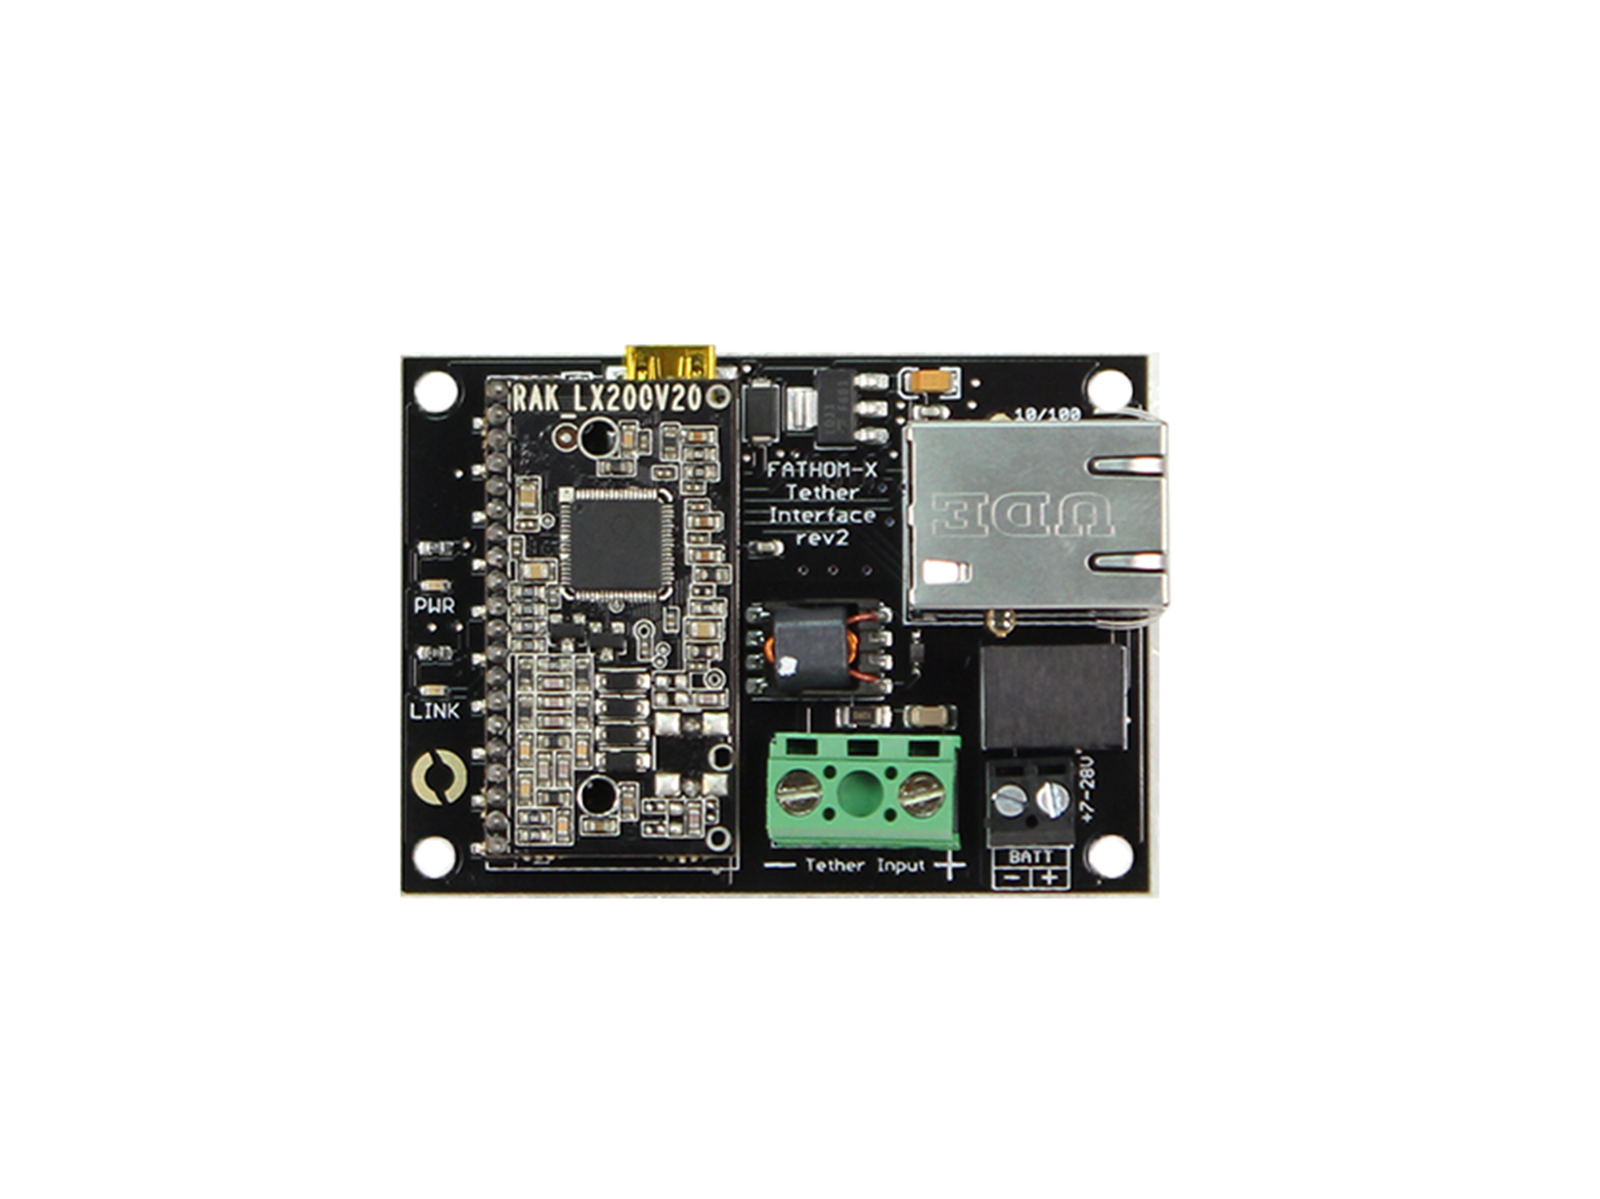
\includegraphics[height=1.8cm, keepaspectratio]{fathom_x.png}
        \hspace{0.2cm}
        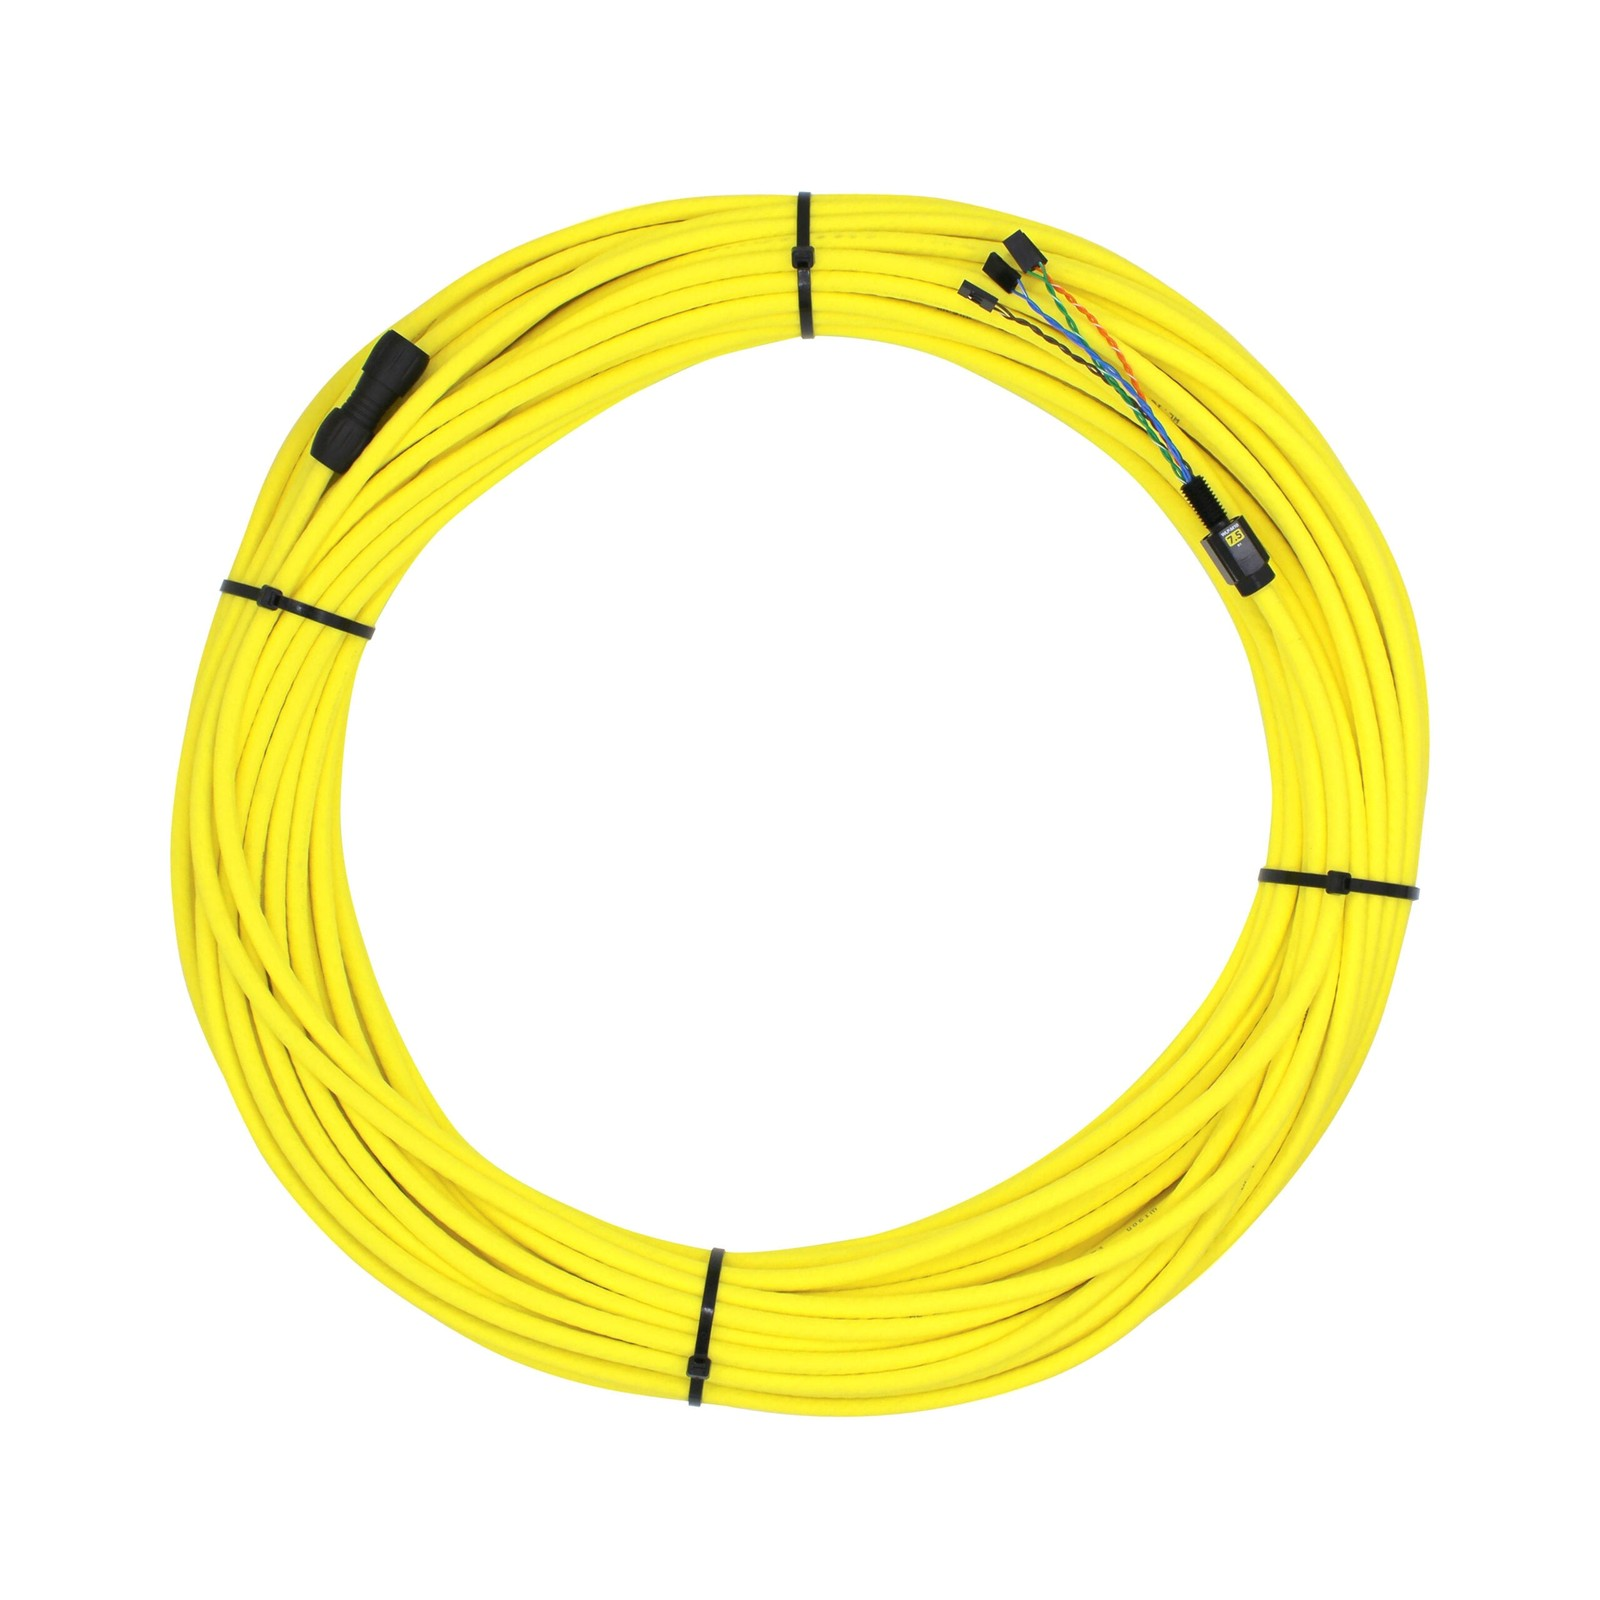
\includegraphics[height=1.8cm, keepaspectratio]{fathom_tether.jpg}\\
        \vspace{0.1em}
        \scriptsize\textbf{Carte Fathom-X} \hspace{0.6cm} \textbf{Ombilical Fathom}\\
        \tiny\textit{CPL HomePlug AV} \hspace{0.5cm} \textit{Flottabilité neutre 300 m}
      \end{center}
      
      \begin{center}
        \begin{tikzpicture}[scale=0.72, every node/.style={transform shape}]
          \node[draw=OceanDeep, fill=OceanDeep!20, rounded corners] (rpi) at (-2,1.2) {\scriptsize RPi 4/5};
          \node[draw=OceanMedium, fill=OceanMedium!20, rounded corners] (fx1) at (-2,0) {\scriptsize Fathom-X};
          \node[draw=OceanMedium, fill=OceanMedium!20, rounded corners] (fx2) at (2,0) {\scriptsize Fathom-X};
          \node[draw=OceanGreen, fill=OceanGreen!20, rounded corners] (pc) at (2,1.2) {\scriptsize PC Surface};
          \draw[<->, thick] (rpi) -- (fx1);
          \draw[<->, line width=1.5pt, OceanCoral] (fx1) -- (fx2) node[midway, above] {\tiny 1 paire 300m};
          \draw[<->, thick] (fx2) -- (pc);
        \end{tikzpicture}
      \end{center}
    \end{column}
  \end{columns}
\end{frame}

\begin{frame}{3.1b Variantes d'Ombilicaux \& Gestion du Câble : Enrouleur de Pont}
  \begin{columns}[T]
    \begin{column}{0.48\textwidth}
      \begin{block}{\tech{Types de Câbles Ombilicaux (Tethers)}}
        \scriptsize
        \begin{itemize}
          \item \textbf{Tether 2 brins (Fathom Standard / Slim)} :
            \begin{itemize}\tiny
              \item 1 paire torsadée Fathom-X ($100\,\text{Mbps}$) + brin central Kevlar.
              \item $\varnothing 7.6\,\text{mm}$ (standard, $150\,\text{kgf}$) vs $\varnothing 4.0\,\text{mm}$ (Slim, traînée $\div 2$).
            \end{itemize}
          \item \textbf{Tether 8 brins (Gigabit High-Bandwidth)} :
            \begin{itemize}\tiny
              \item 4 paires blindées ($1000\,\text{Mbps}$) pour flux 4K \& sonars lourds.
            \end{itemize}
        \end{itemize}
      \end{block}

      \vspace{0.2em}
      \begin{center}
        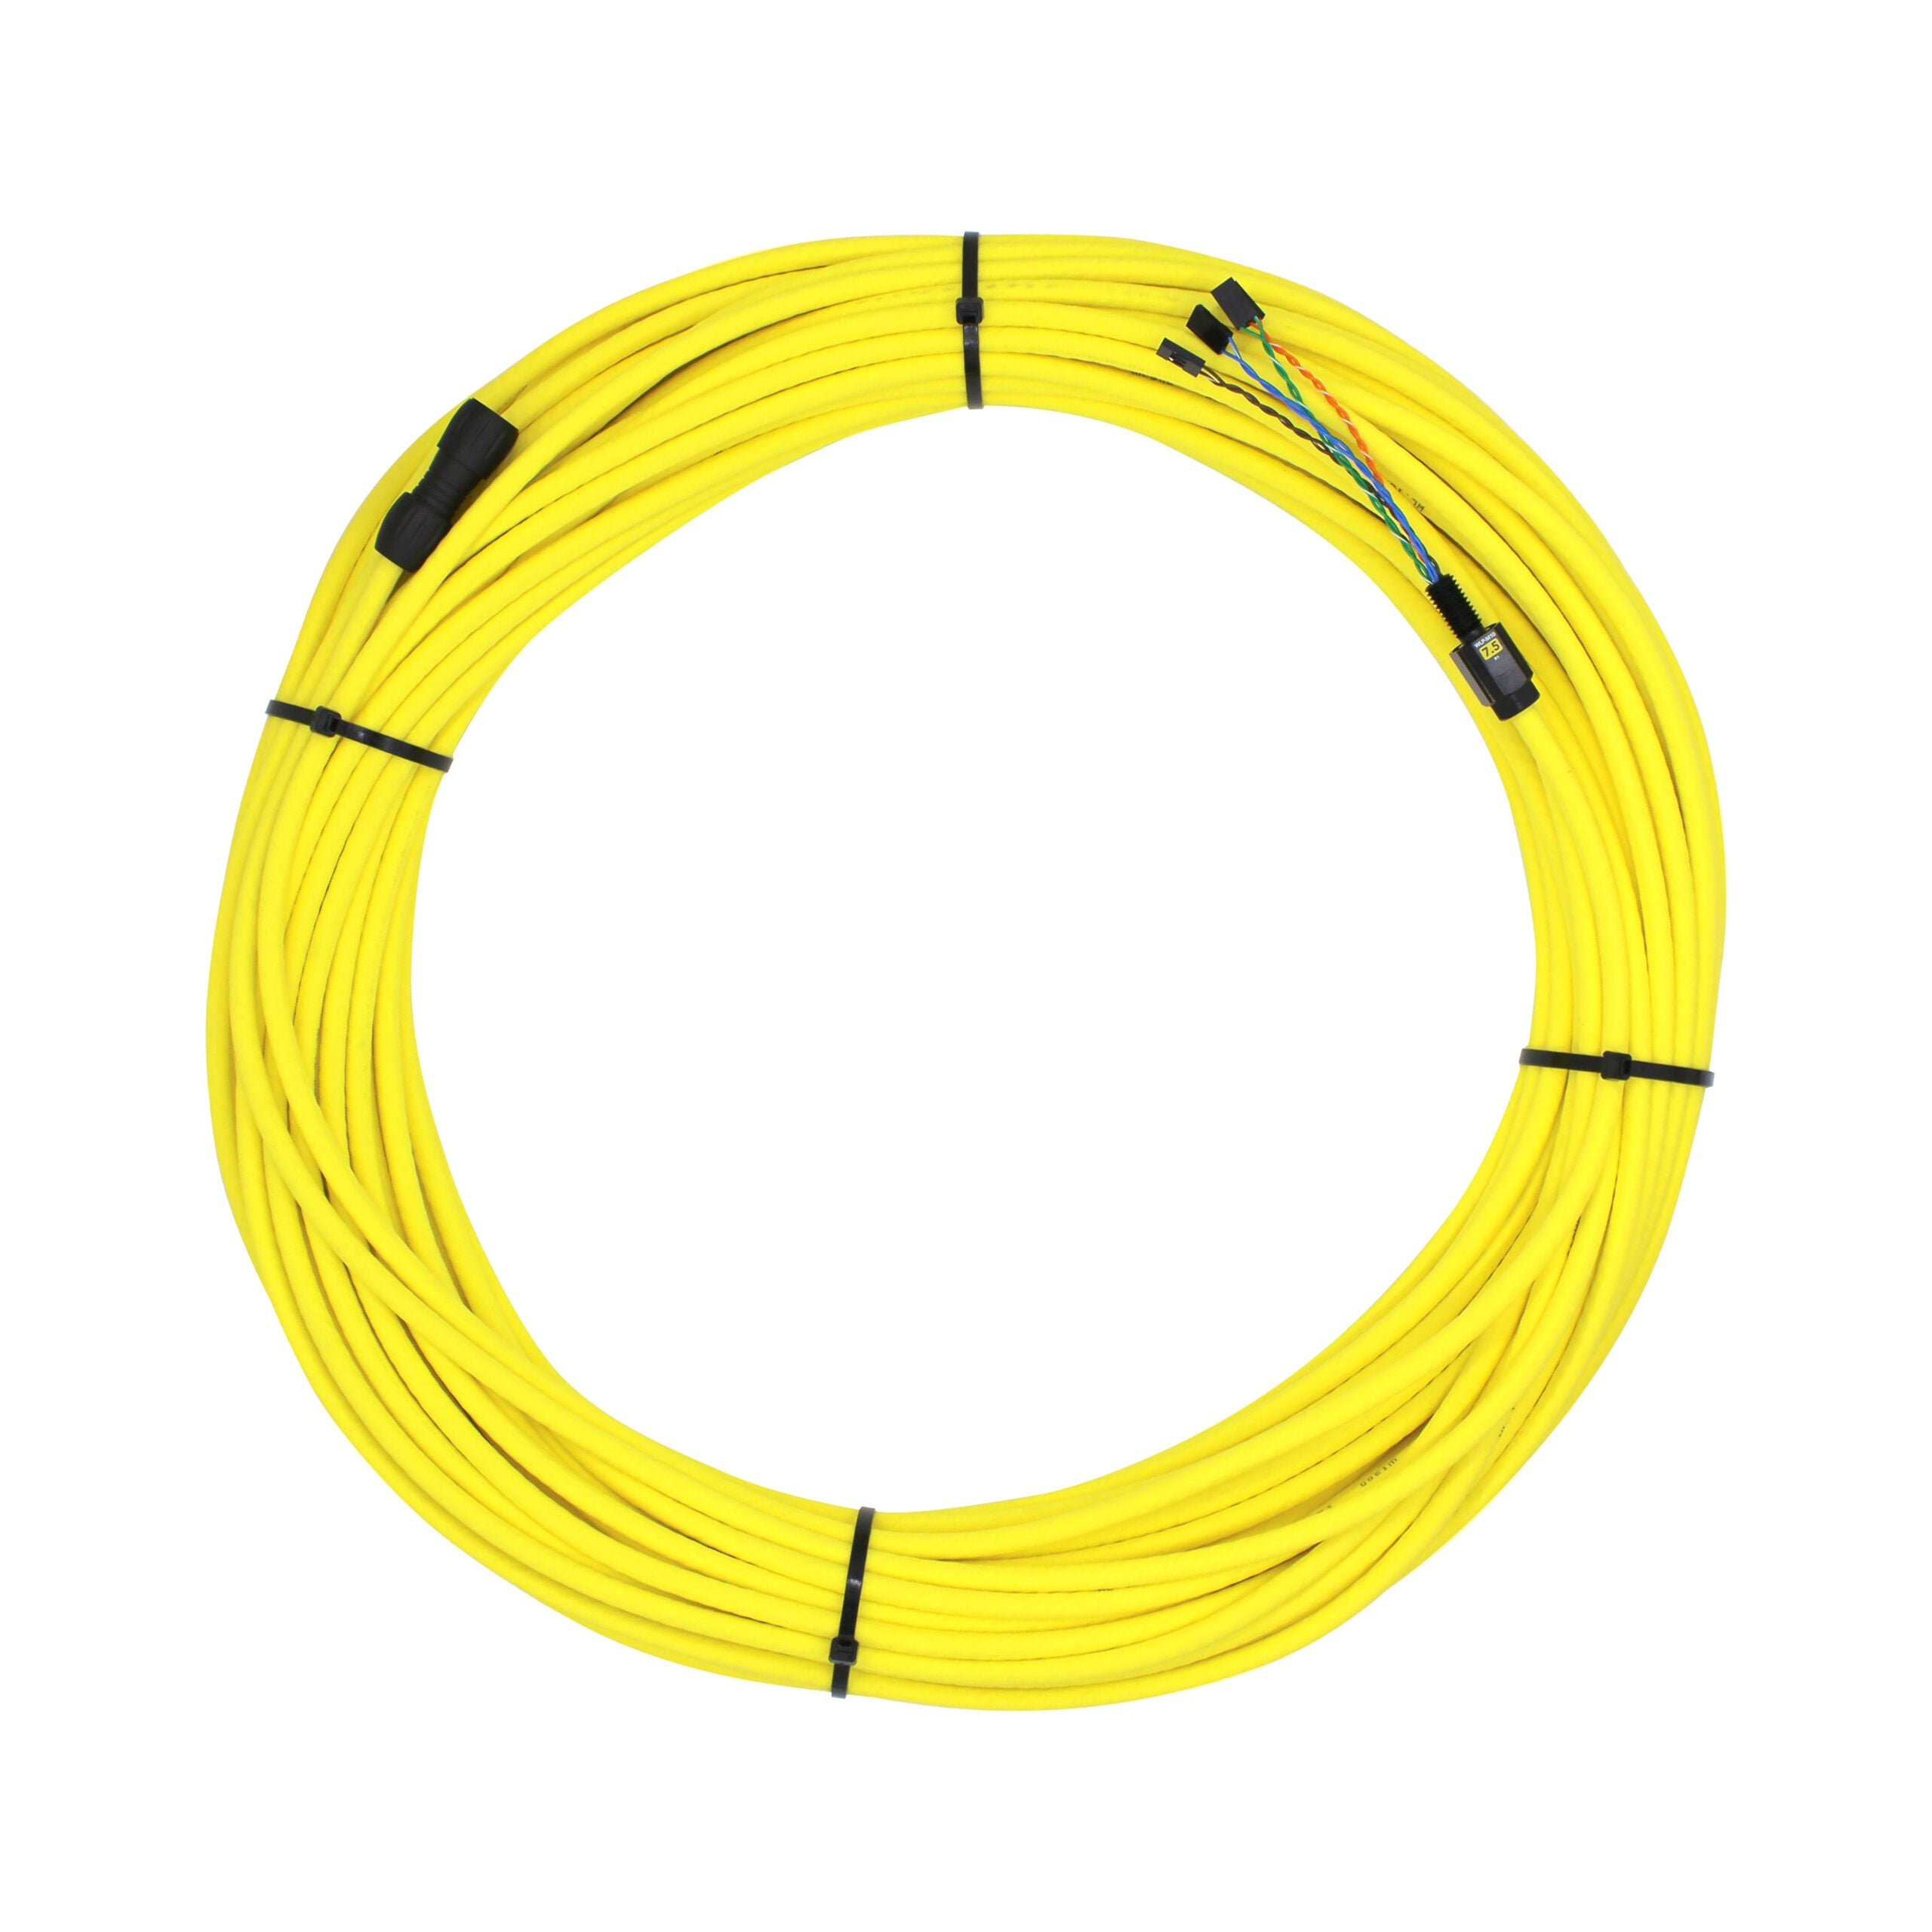
\includegraphics[height=1.4cm, keepaspectratio]{tether_standard_photo.jpg}
        \hspace{0.2cm}
        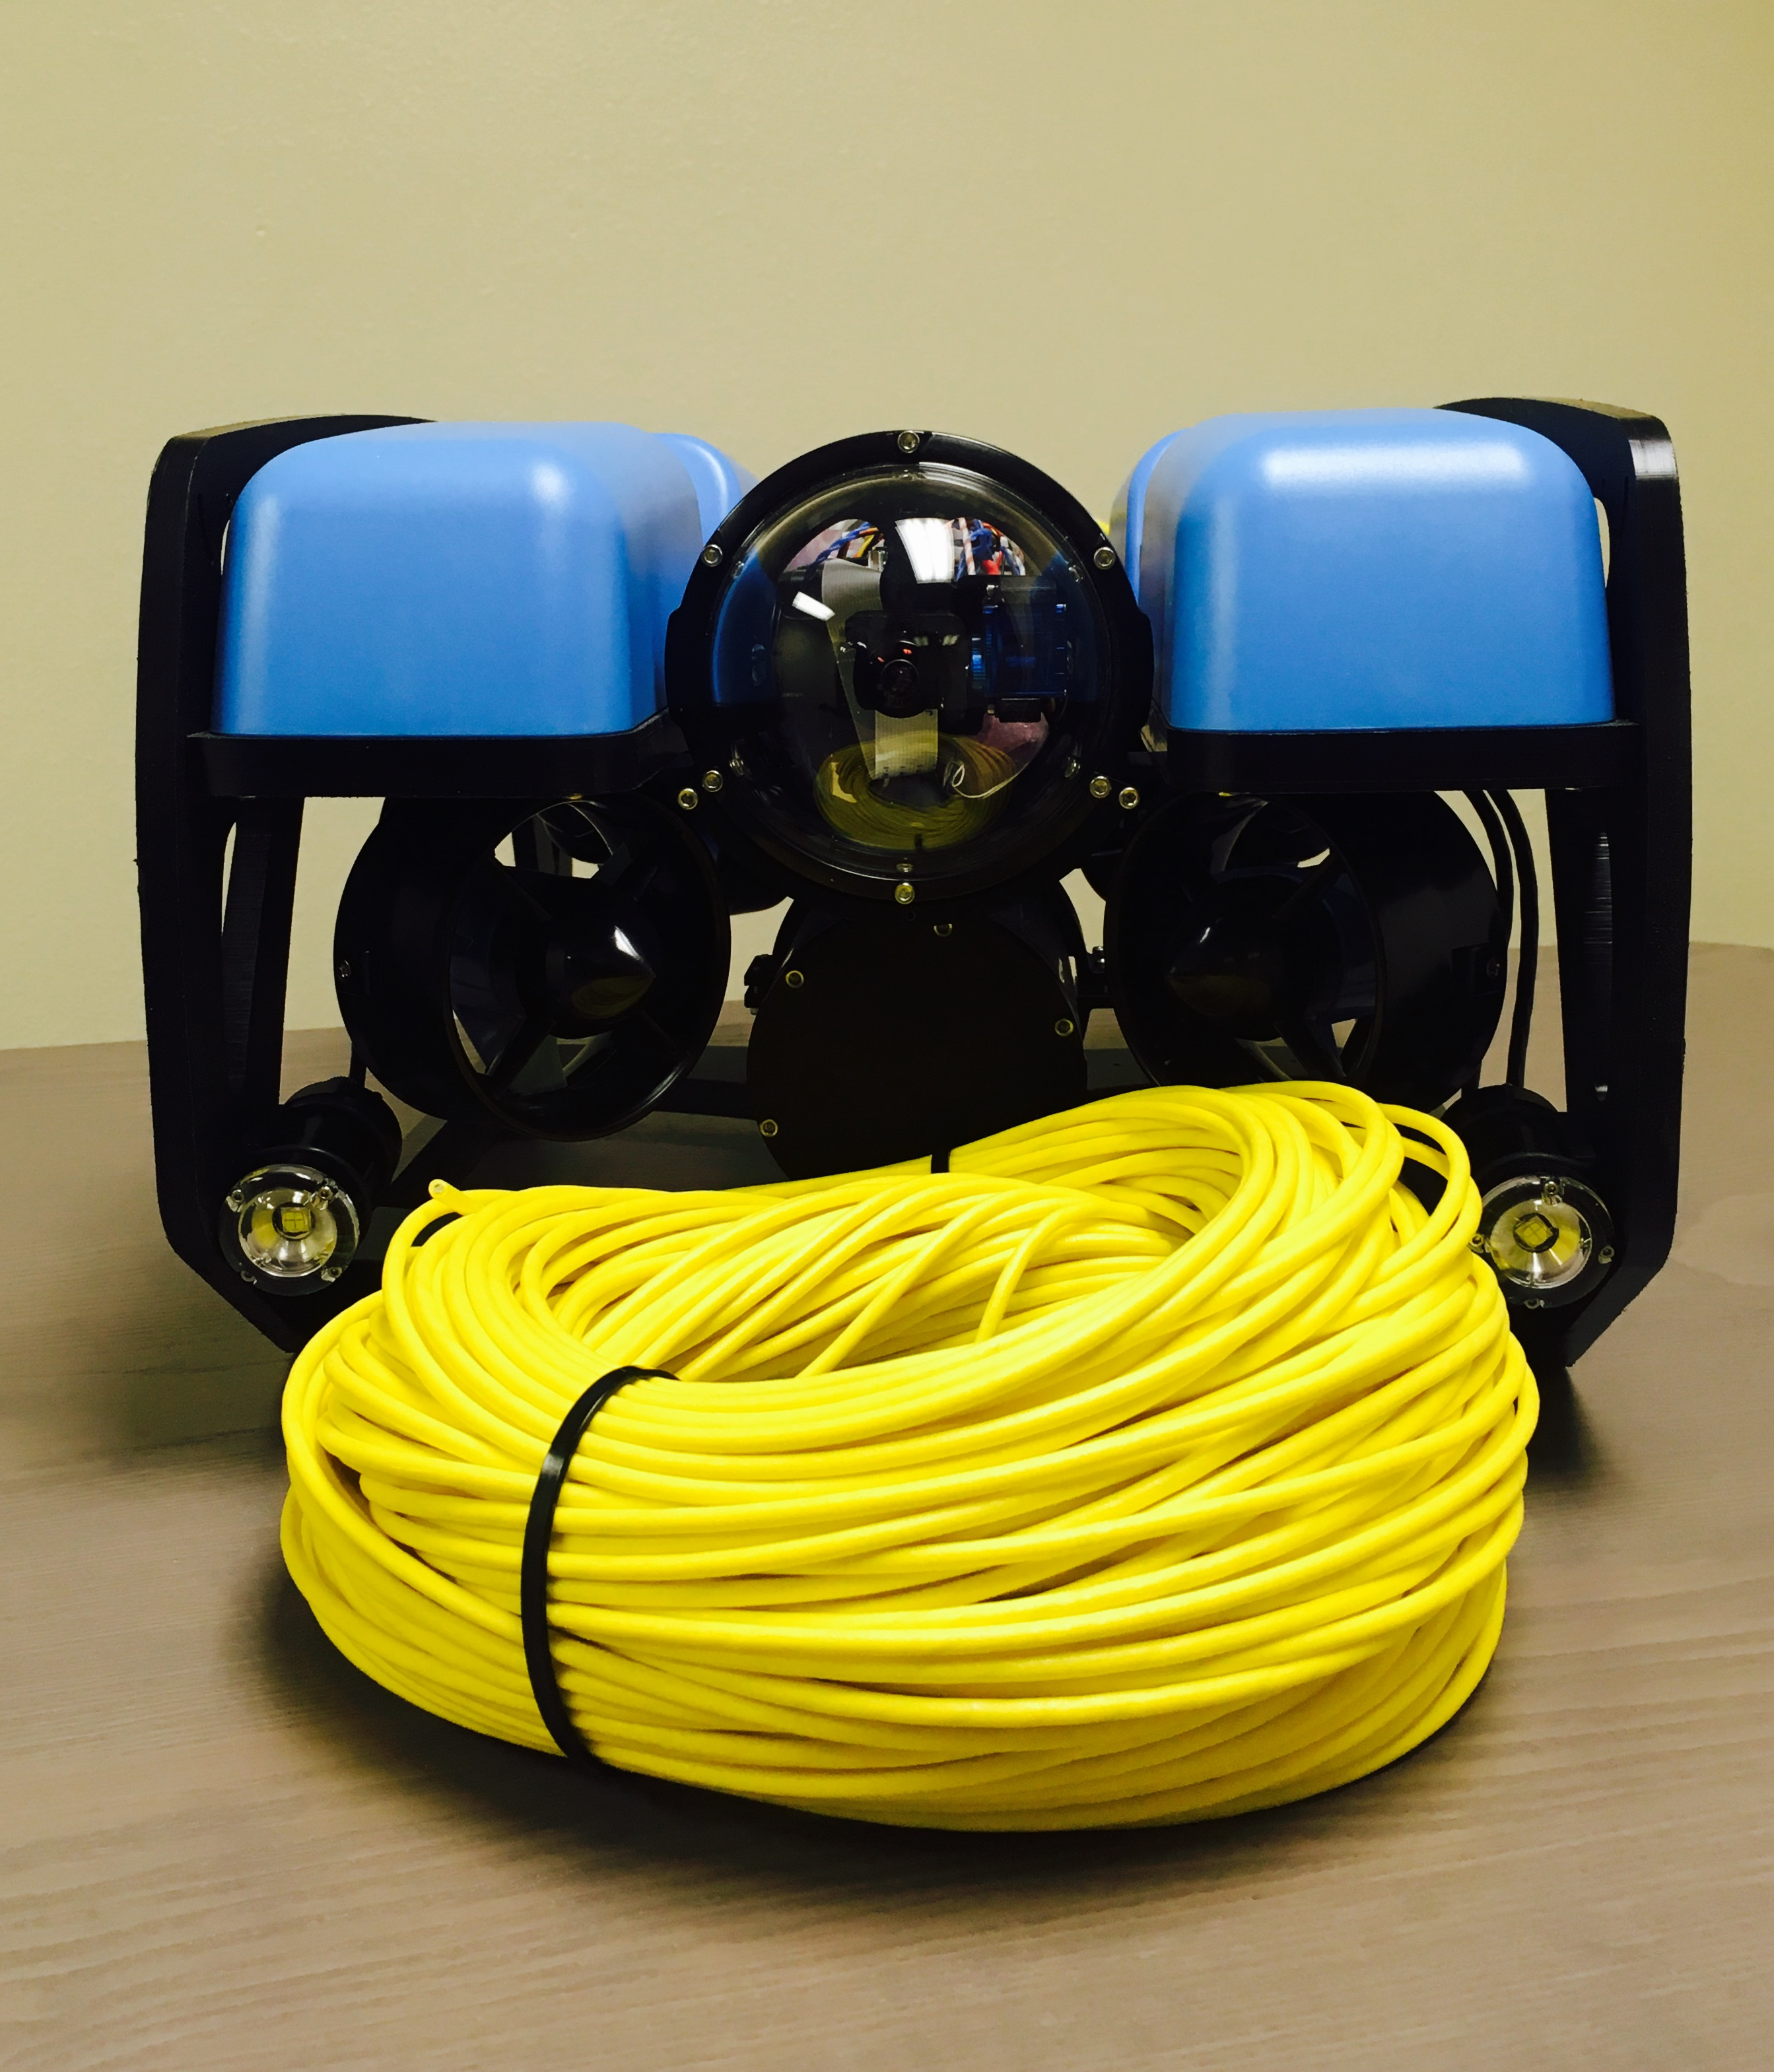
\includegraphics[height=1.4cm, keepaspectratio]{tether_slim_photo.jpg}\\
        \vspace{0.1em}
        \tiny\textbf{Ombilical Standard ($\varnothing 7.6\,\text{mm}$)} \hspace{0.3cm} \textbf{Ombilical Slim ($\varnothing 4.0\,\text{mm}$)}
      \end{center}
    \end{column}

    \begin{column}{0.50\textwidth}
      \begin{block}{\succw{L'Enrouleur de Pont avec Collecteur Tournant (*Slip Ring*)}}
        \scriptsize
        \begin{itemize}
          \item \textbf{Gestion des $300\,\text{m}$ de câble} : déroulage et virage sous tension sans vrille.
          \item \textbf{Joint tournant électro-optique / slip ring} : transfert continu des signaux haute fréquence ($100\text{--}1000\,\text{Mbps}$) pendant la rotation du touret.
        \end{itemize}
      \end{block}

      \vspace{0.2em}
      \begin{center}
        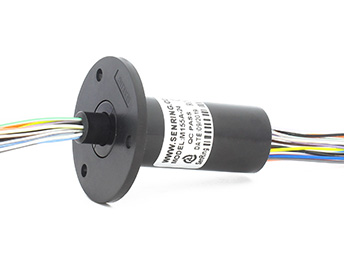
\includegraphics[height=1.4cm, keepaspectratio]{slip_ring.jpg}
        \hspace{0.3cm}
        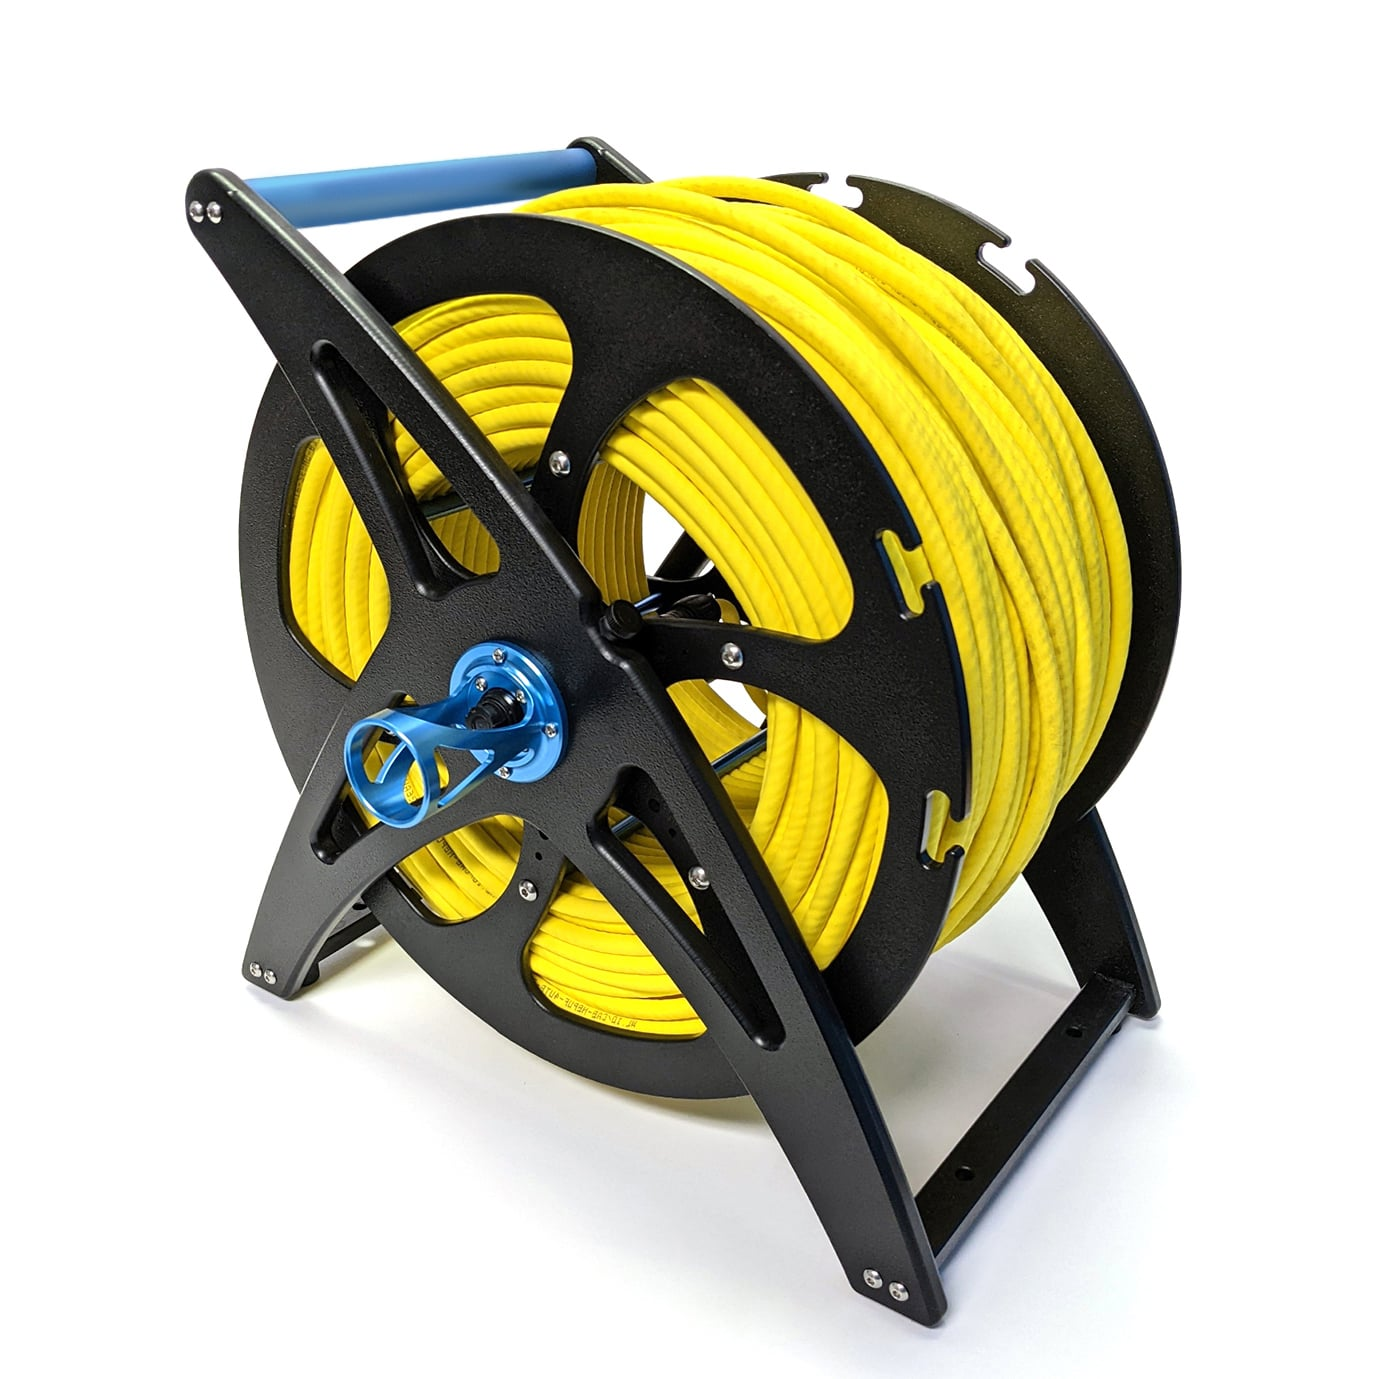
\includegraphics[height=1.4cm, keepaspectratio]{fathom_spool.jpg}\\
        \vspace{0.1em}
        \tiny\textbf{Collecteur tournant (*Slip Ring*)} \hspace{0.3cm} \textbf{Enrouleur de pont}
      \end{center}
    \end{column}
  \end{columns}
\end{frame}

\begin{frame}{3.1b Architecture des Essais : Station Sol, FXTI, BaseStation \& RC}
  \begin{columns}[c]
    \begin{column}{0.48\textwidth}
      \begin{center}
        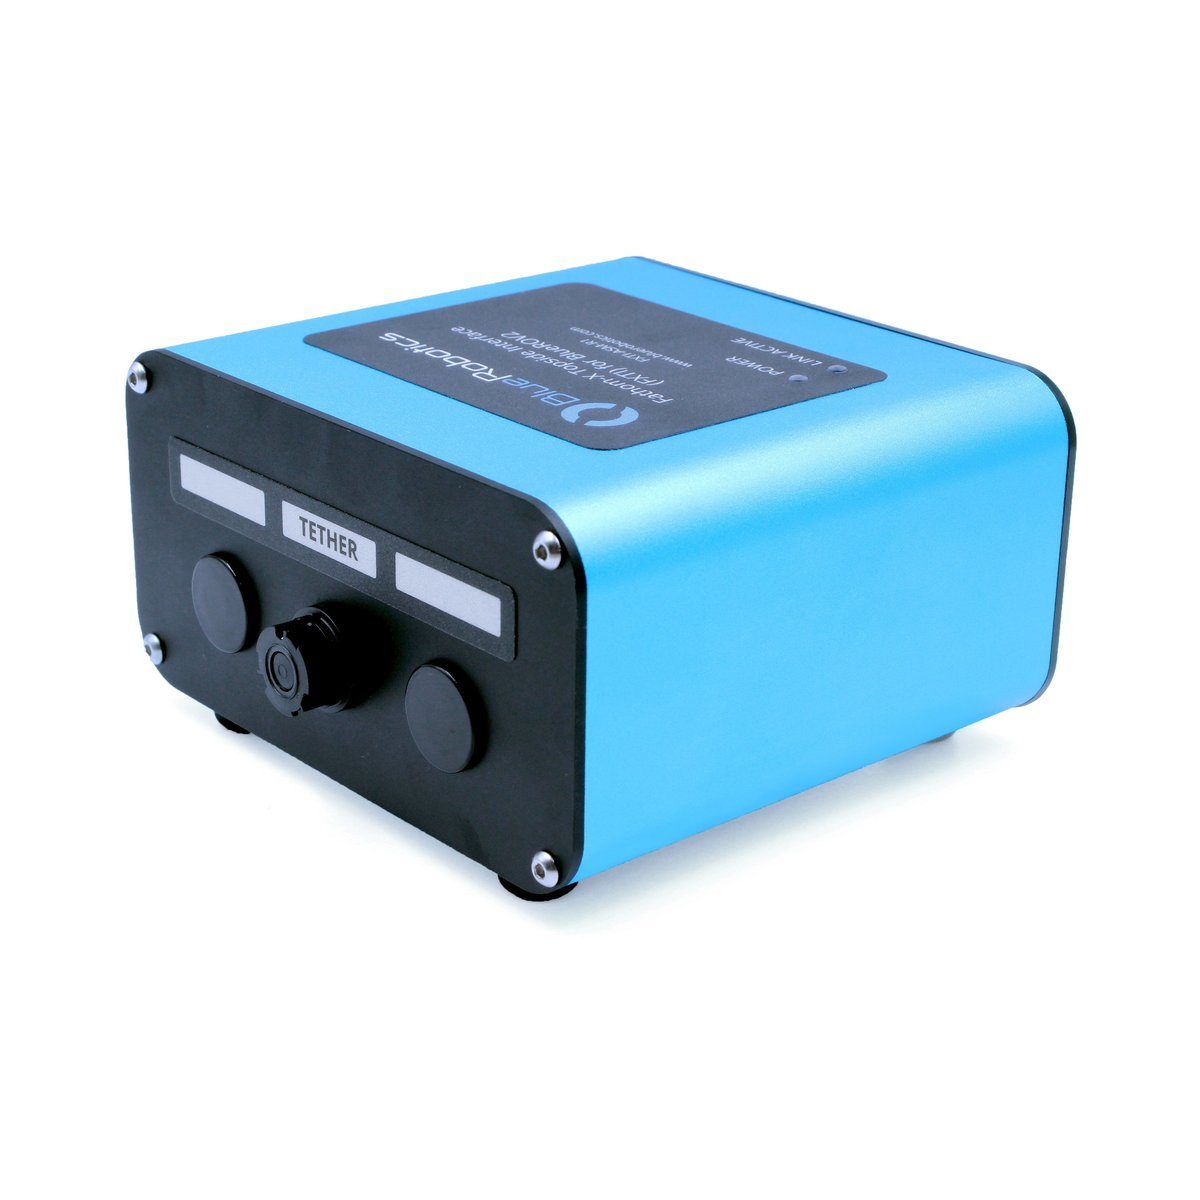
\includegraphics[height=1.5cm, keepaspectratio]{fxti_interface.jpg}
        \hspace{0.2cm}
        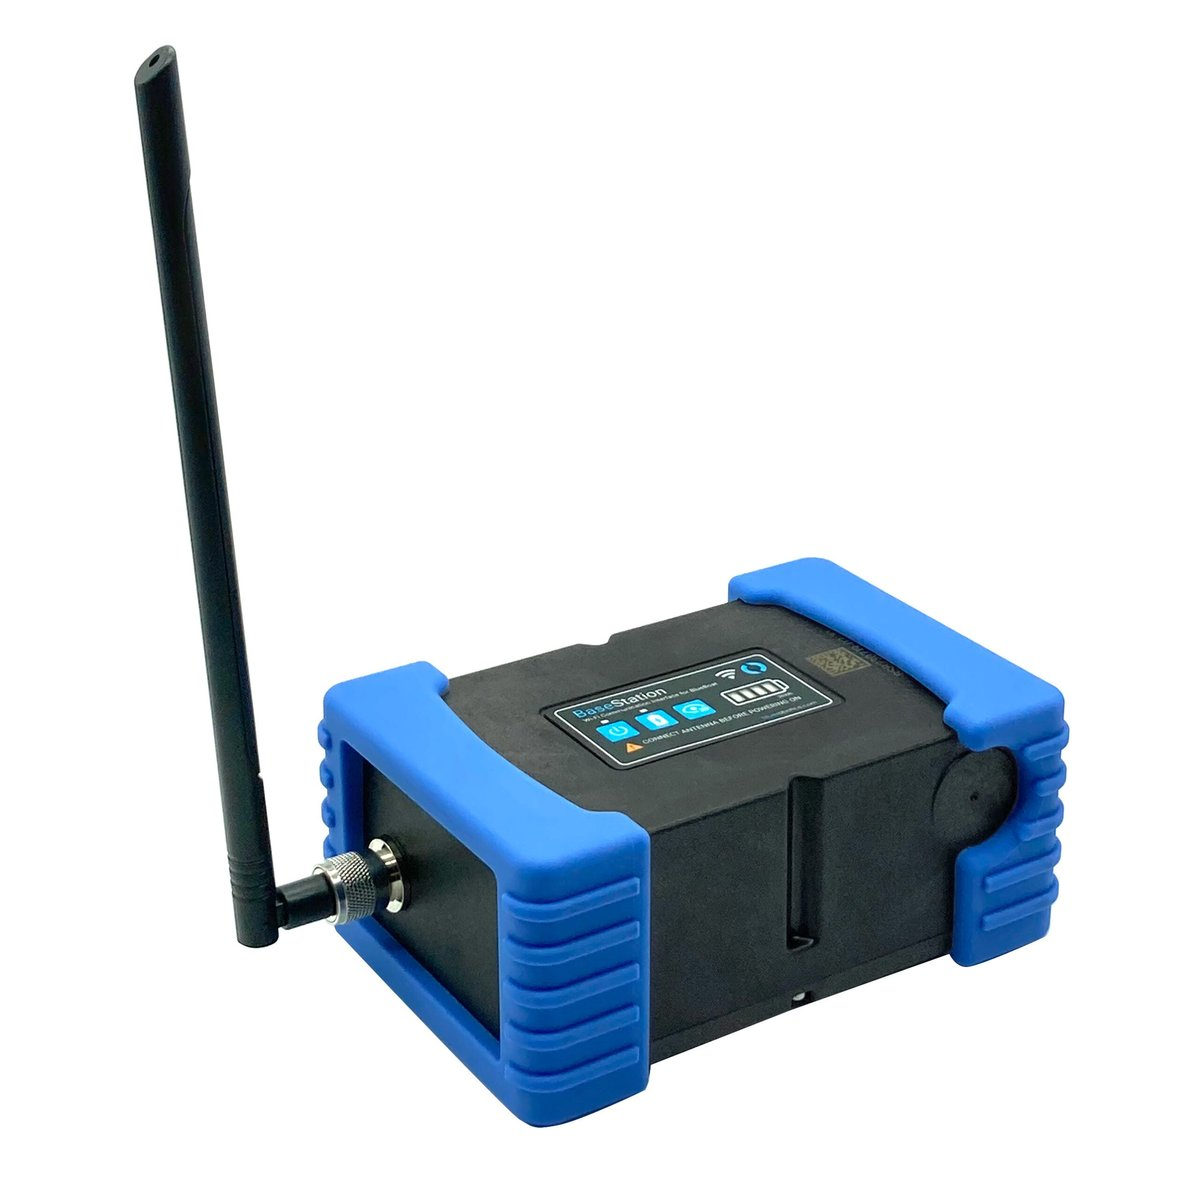
\includegraphics[height=1.5cm, keepaspectratio]{basestation_wifi.jpg}\\
        \vspace{0.1em}
        \tech{Boîtier FXTI (ROV)} \hspace{0.6cm} \succw{BaseStation WiFi (ASV)}\\
        \tiny\textit{Interface ombilical Fathom-X} \hspace{0.4cm} \textit{MikroTik 2.4 GHz longue portée}
      \end{center}
      \scriptsize
      \begin{block}{\tech{Poste de Contrôle Surface (GCS)}}
        PC durci quai/navire avec joystick USB :
        \begin{itemize}
          \item \textbf{QGroundControl} ou navigateur \textbf{Cockpit}.
          \item Visualisation télémétrie, vidéo HD, alertes.
        \end{itemize}
      \end{block}
    \end{column}

    \begin{column}{0.50\textwidth}
      \scriptsize
      \begin{block}{\tech{ROV Sous-Marin : Liaison Ombilicale}}
        \begin{itemize}
          \item Ombilical Fathom relié au boîtier \textbf{FXTI}.
          \item CPL HomePlug AV vers USB/Ethernet ($100\,\text{Mbps}$).
        \end{itemize}
      \end{block}

      \begin{block}{\succw{ASV Surface (BlueBoat) : WiFi \& Sécurité RC}}
        \begin{itemize}
          \item \textbf{BaseStation WiFi} : antenne 2.4 GHz ($>1\,\text{km}$).
          \item \alertw{Radiocommande RC manuelle (2.4 GHz SBUS)} :
            \begin{itemize}
              \item Récepteur RC direct sur le Navigator.
              \item Pilotage à vue pour mise à l'eau / quai.
              \item Sécurité matérielle immédiate (*kill-switch*).
            \end{itemize}
        \end{itemize}
      \end{block}
    \end{column}
  \end{columns}
\end{frame}

\begin{frame}{3.1c Transport d'Énergie Haute Tension : Système OTPS}
  \begin{columns}[c]
    \begin{column}{0.48\textwidth}
      \begin{center}
        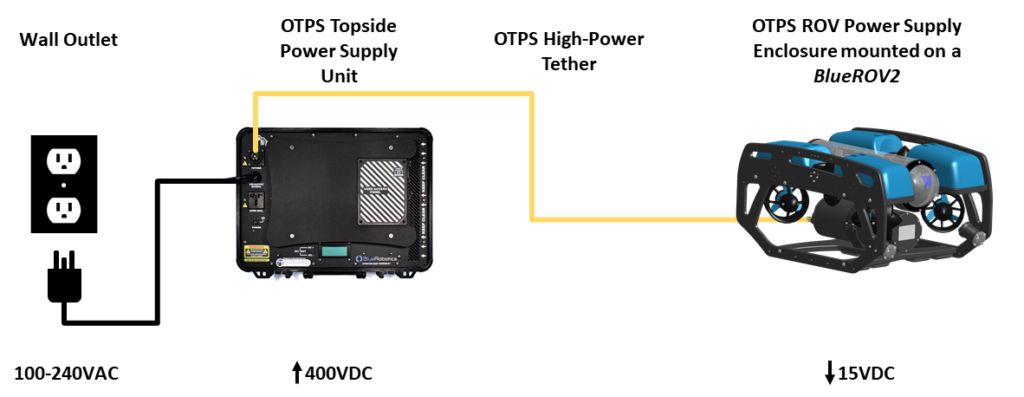
\includegraphics[width=\textwidth, height=2.8cm, keepaspectratio]{otps_power_system.png}\\
        \vspace{0.2em}
        \tech{Système OTPS (Outland Technology Power Supply)}\\
        \scriptsize\textit{Transport 400V DC par ombilical \& abaissement 15V sous-marin}
      \end{center}
      \scriptsize
      \begin{alertblock}{La Limite des Batteries}
        Autonomie limitée à $2\text{--}4\,\text{h}$. Remplacement de batterie fastidieux obligeant à sortir et sécher le robot.
      \end{alertblock}
    \end{column}

    \begin{column}{0.50\textwidth}
      \textbf{La physique du transport haute tension} :
      \scriptsize
      \begin{itemize}
        \item Puissance transportée : $P = U \cdot I$.
        \item Pour transmettre $1000\,\text{W}$ sur $300\,\text{m}$ :
          \begin{itemize}
            \item En basse tension ($15\,\text{V}$) : $I \approx 67\,\text{A}$ $\rightarrow$ pertes Joule destructrices ($P = R I^2$).
            \item En haute tension (\succw{$400\,\text{V DC}$}) : $I \approx 2.5\,\text{A}$ !
          \end{itemize}
        \item Pertes Joule divisées par $(400/15)^2 \approx \succw{700}$ !
      \end{itemize}

      \vspace{0.2em}
      \begin{block}{\succw{Architecture Électronique Embarquée}}
        \begin{itemize}
          \item \textbf{Boîtier Surface} : redresse le secteur $110/240\,\text{V AC}$ vers $400\,\text{V DC}$ régulé.
          \item \textbf{Carte de Puissance Sous-Marine} : hacheur abaisseur DC-DC isolé dans le caisson du ROV, convertissant le $400\,\text{V DC}$ en \textbf{$15\,\text{V DC}$ continu (jusqu'à $45\,\text{A}$ / $1000\,\text{W}$)}.
          \item Permet des plongées illimitées (24h/24) !
        \end{itemize}
      \end{block}
    \end{column}
  \end{columns}
\end{frame}

\begin{frame}{3.2 Le C{\oe}ur Logiciel Moderne : L'Écosystème BlueOS}
  \begin{columns}[T]
    \begin{column}{0.5\textwidth}
      \begin{block}{\tech{Qu'est-ce que BlueOS ?}}
        \begin{itemize}
          \item Le système d'exploitation embarqué moderne de BlueRobotics (remplaçant historique du script Python \textit{companion}).
          \item Tourne sur le \textbf{Raspberry Pi 4 / 5} (base Linux Debian).
          \item Architecture entièrement conteneurisée via \textbf{Docker} :
            \begin{itemize}
              \item Service vidéo WebRTC / RTSP ultra-faible latence.
              \item Routeur MAVLink centralisé (MAVLink2Rest).
              \item Flasheur de firmware d'autopilote en un clic.
            \end{itemize}
        \end{itemize}
      \end{block}
    \end{column}

    \begin{column}{0.5\textwidth}
      \begin{block}{\succw{Avantages Clés pour le Scientifique}}
        \begin{itemize}
          \item \textbf{Zéro logiciel à installer en surface} : accessible depuis un simple navigateur web sur \code{http://blueos.local} ou \code{192.168.2.2}.
          \item Gestionnaire de fichiers web pour télécharger les logs directement.
          \item Terminal SSH interactif intégré dans l'interface web.
          \item Monitoring complet : température CPU, tension d'alimentation, usage mémoire.
        \end{itemize}
      \end{block}
    \end{column}
  \end{columns}
\end{frame}

\begin{frame}{3.3 Le Magasin d'Extensions BlueOS pour la Recherche}
  \begin{columns}[c]
    \begin{column}{0.55\textwidth}
      \textbf{Comment intégrer vos propres capteurs ?}
      \begin{itemize}
        \item BlueOS dispose d'un gestionnaire d'\textbf{Extensions conteneurisées} (similaire à un "App Store" de bord).
        \item N'importe quel chercheur ou ingénieur peut créer son conteneur Docker avec un script Python de lecture de capteur (sonde CTD, fluorimètre, sonar).
        \item L'extension peut exposer :
          \begin{itemize}
            \item Une page web dédiée dans BlueOS.
            \item Des flux de données MAVLink personnalisés.
            \item Un broker de données partagé.
          \end{itemize}
        \item Installation et mise à jour en 1 clic sans risque de corrompre le système de base du drone.
      \end{itemize}
    \end{column}

    \begin{column}{0.45\textwidth}
      \begin{block}{Extensions Déjà Disponibles}
        \begin{itemize}
          \item \tech{Ping Viewer} : visualisation sonar Ping / Ping360.
          \item \tech{DVL Extension} : driver et interface Water Linked DVL-A50.
          \item \tech{NMEA Injector} : injection de GPS de surface vers l'autopilote.
          \item \tech{Node-RED} : automatisation de flux de données sans coder.
          \item \tech{ROS 2 Bridge} : communication native avec l'écosystème robotique.
        \end{itemize}
      \end{block}
    \end{column}
  \end{columns}
\end{frame}

\begin{frame}{3.4 Interfaces de Contrôle : QGroundControl vs Cockpit}
  \begin{columns}[T]
    \begin{column}{0.48\textwidth}
      \begin{center}
        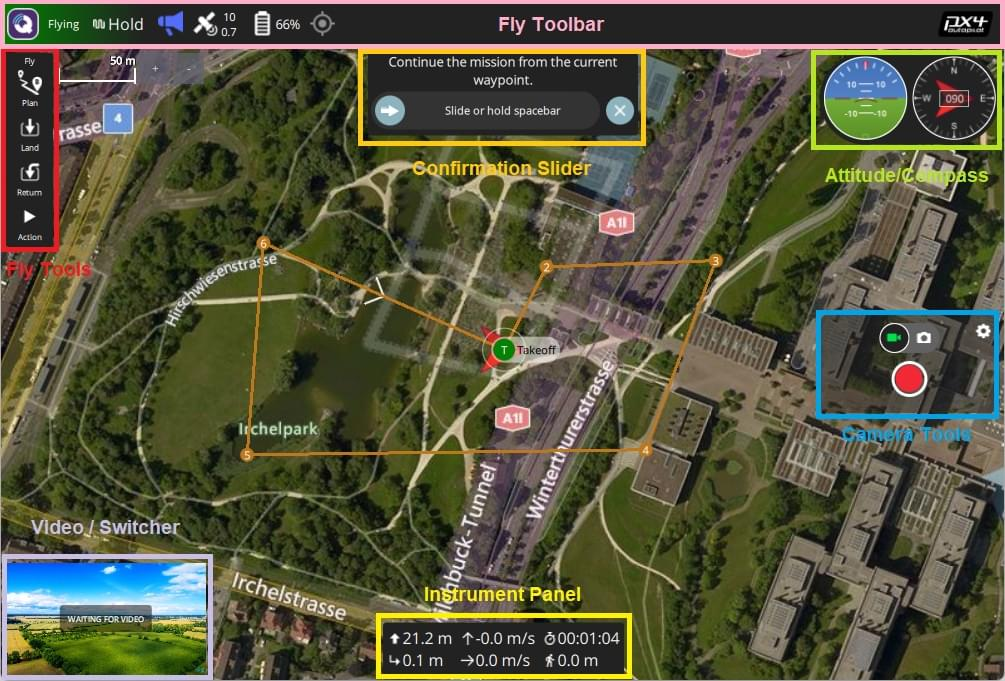
\includegraphics[width=\linewidth, height=2.45cm, keepaspectratio]{qgroundcontrol_interface.jpg}\\
        \vspace{0.15em}
        \tech{QGroundControl (QGC)}\\
        \tiny\textit{Station sol native (C++ / Qt) --- Vue Télémétrie \& HUD}
      \end{center}
      \vspace{-0.4em}
      \begin{block}{QGroundControl : Le Standard Éprouvé}
        \scriptsize
        \begin{itemize}
          \item \textbf{Application native historique} (15 ans) : multiplateforme (PC, Mac, Linux, tablettes).
          \item \textbf{Fonctions} : calibrage joysticks/capteurs, incrustation vidéo HUD, planification de waypoints.
          \item \alertw{Limite} : rigide, difficile d'intégrer des widgets pour sondes océanographiques sur-mesure.
        \end{itemize}
      \end{block}
    \end{column}

    \begin{column}{0.48\textwidth}
      \begin{center}
        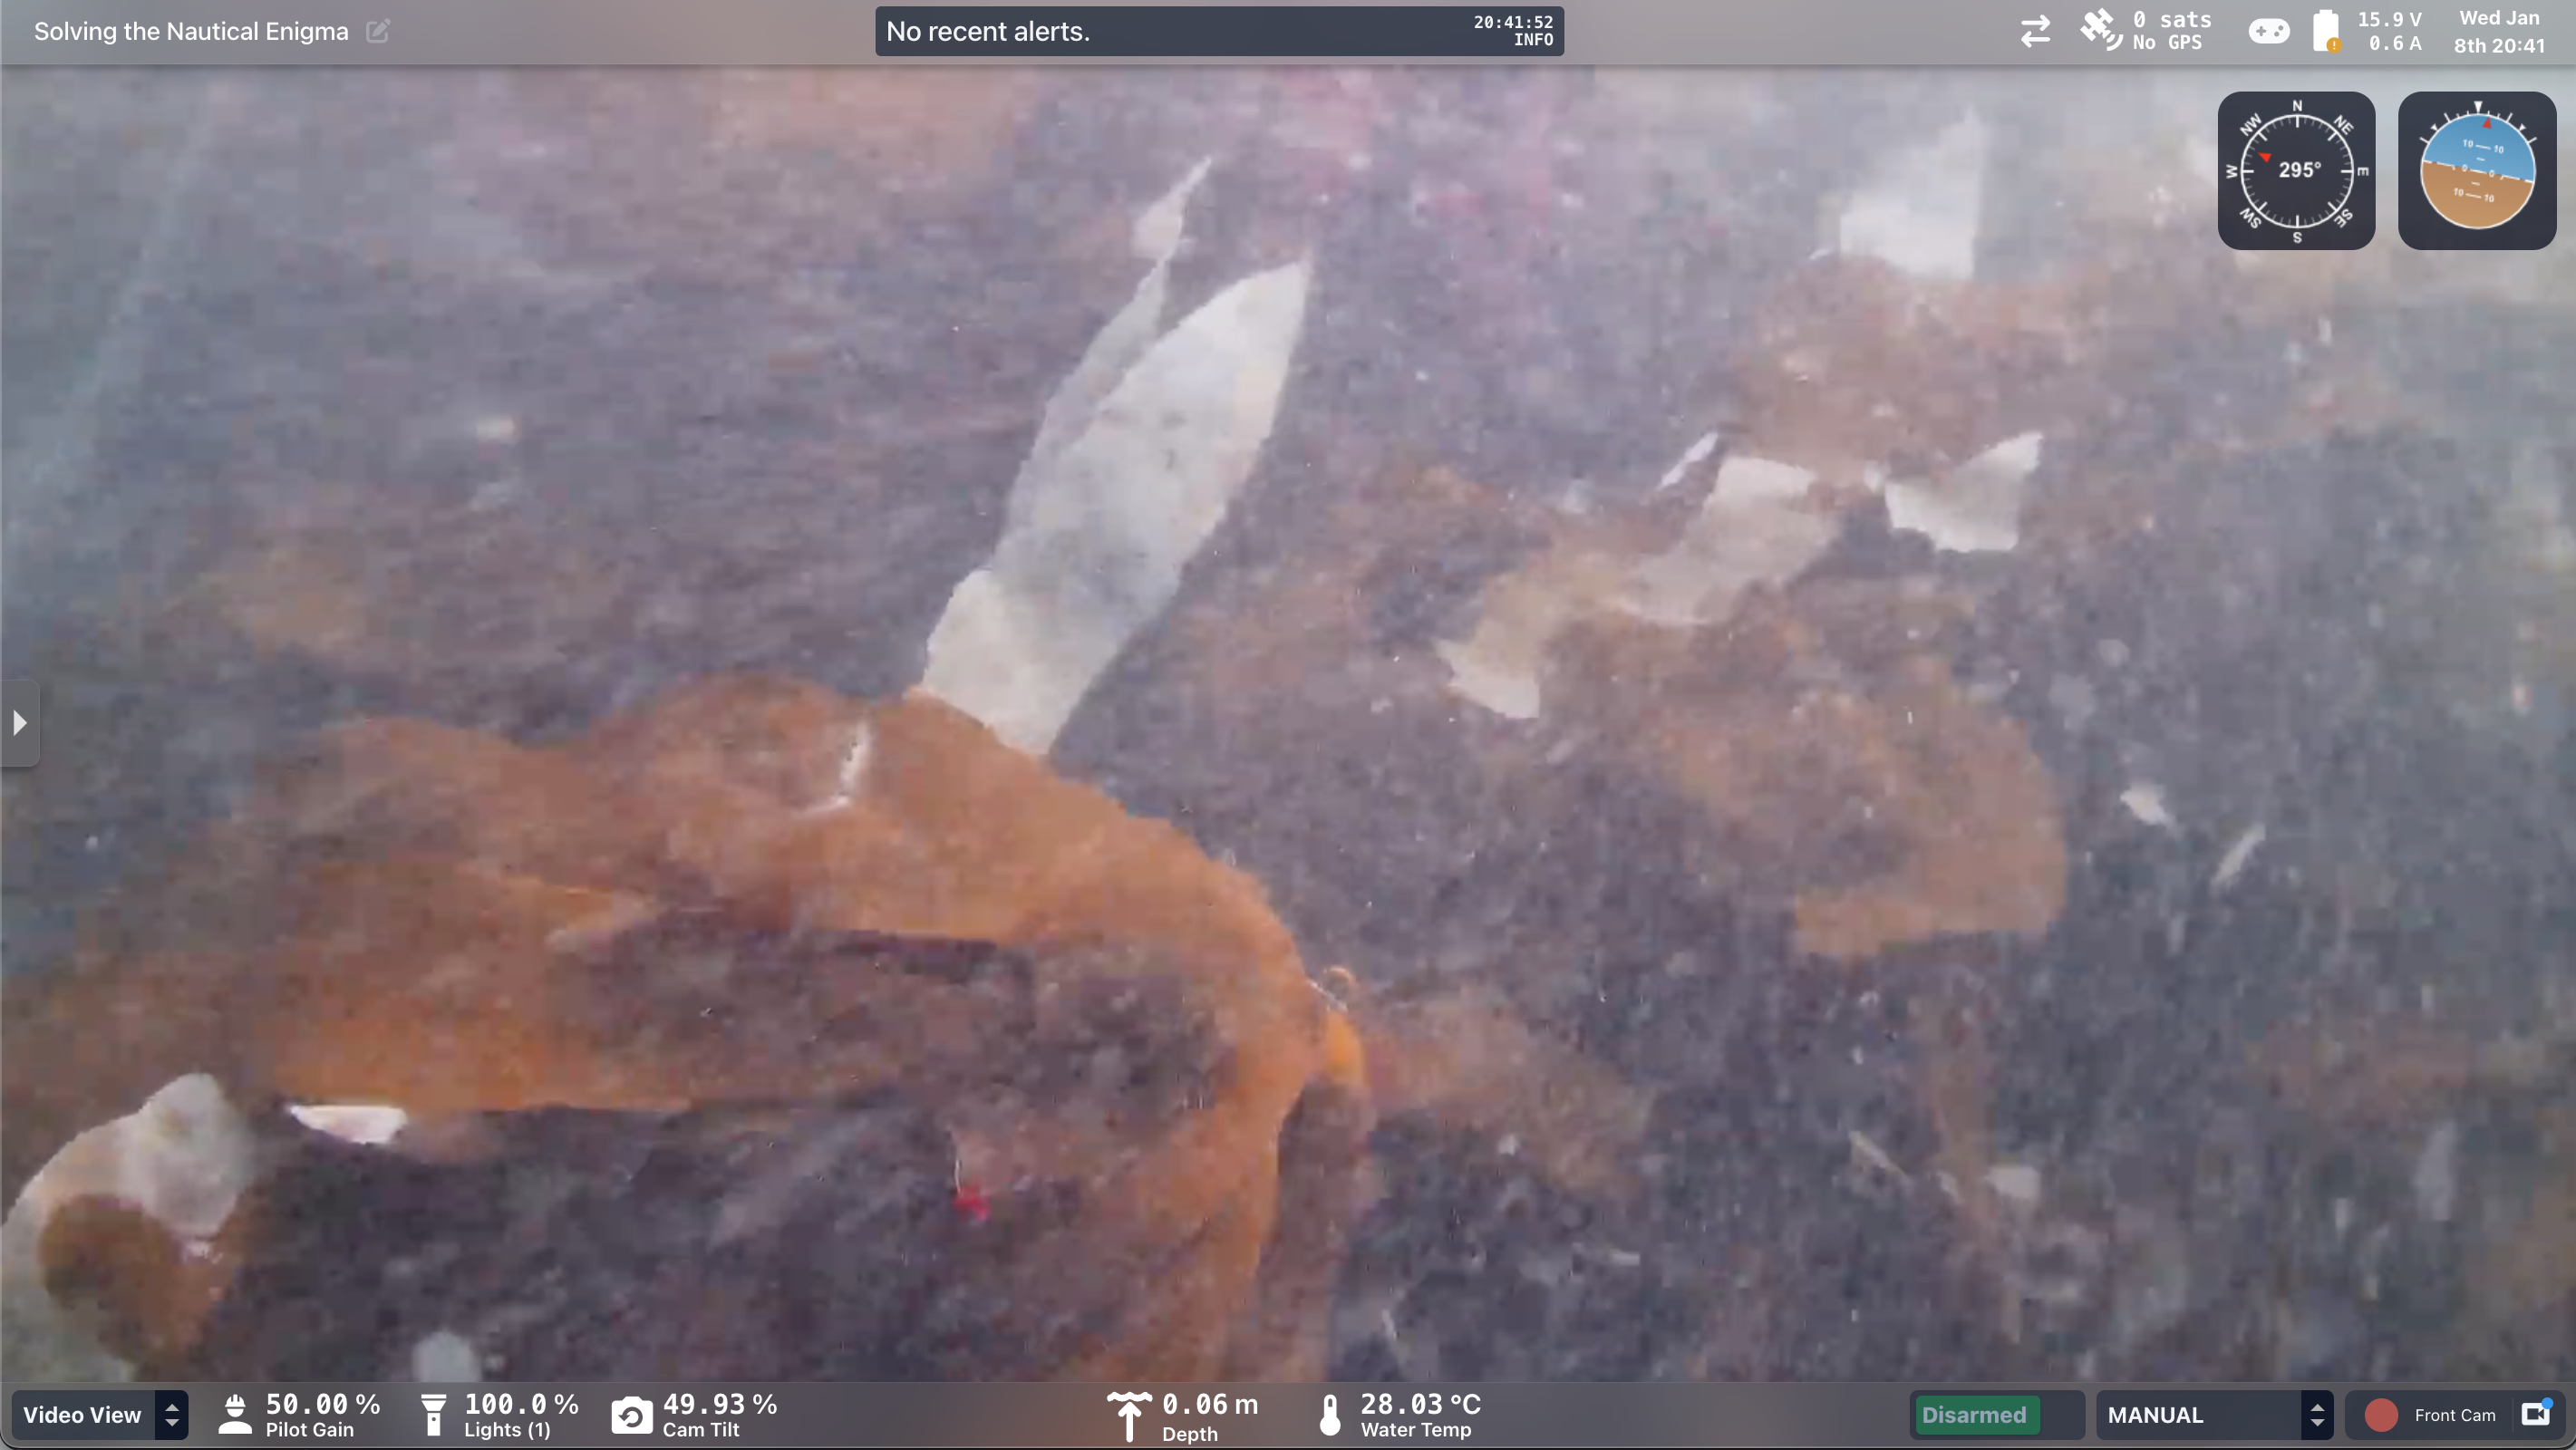
\includegraphics[width=\linewidth, height=2.45cm, keepaspectratio]{sub-video-view.png}\\
        \vspace{0.15em}
        \succw{Cockpit (BlueRobotics)}\\
        \tiny\textit{Interface web moderne (HTML5 / Vue.js) --- Vue Vidéo ROV}
      \end{center}
      \vspace{-0.4em}
      \begin{block}{Cockpit : La Nouvelle Génération Web}
        \scriptsize
        \begin{itemize}
          \item \textbf{Zéro installation client} : tourne directement dans le navigateur (Chrome / Firefox) via BlueOS.
          \item \textbf{100\% modulaire} : organisation des vues et panneaux en glisser-déposer (\textit{drag \& drop}).
          \item \succw{Personnalisable} : développement facile de widgets scientifiques (sonde CTD, sonar, etc.).
        \end{itemize}
      \end{block}
    \end{column}
  \end{columns}
\end{frame}

\begin{frame}{3.4b Cockpit en Pratique : Vues Métier Dédiées (ROV vs ASV)}
  \begin{columns}[T]
    \begin{column}{0.48\textwidth}
      \begin{center}
        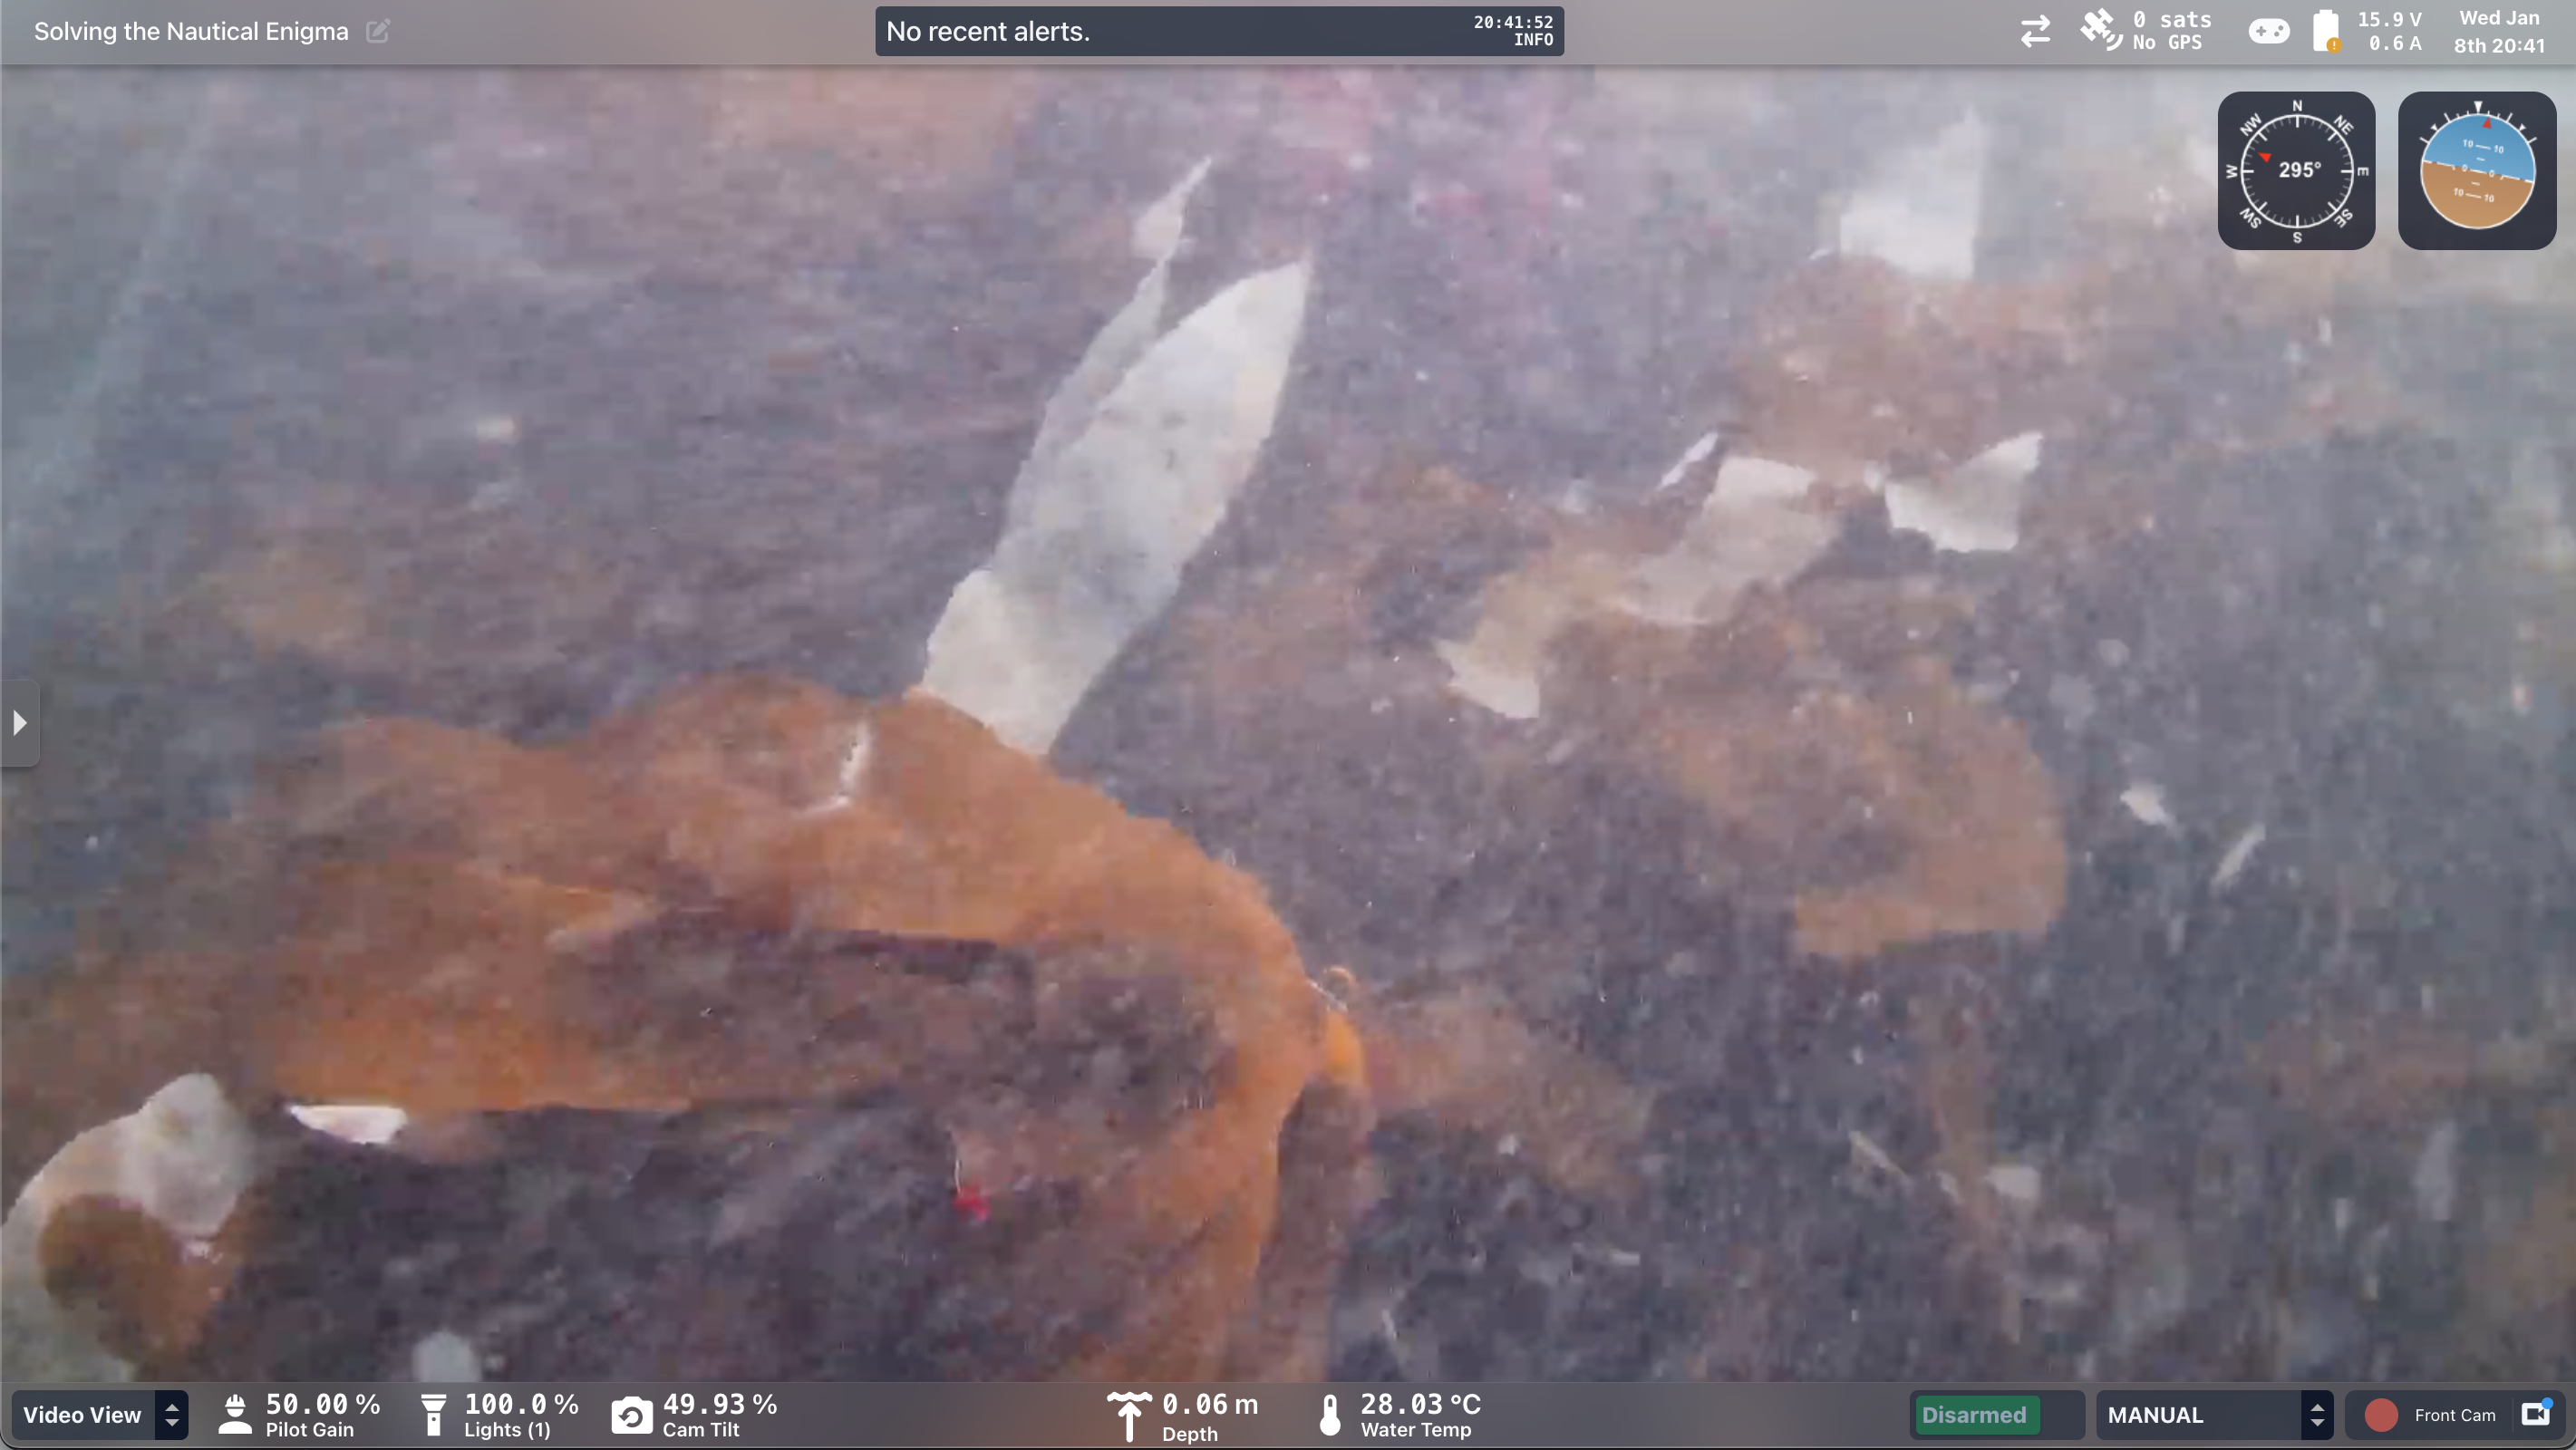
\includegraphics[width=\linewidth, height=2.35cm, keepaspectratio]{sub-video-view.png}\\
        \vspace{0.15em}
        \tech{Vue Vidéo \& Pilotage ROV (BlueROV2)}\\
        \tiny\textit{Inspection subaquatique, capteurs de sûreté et commandes directes}
      \end{center}
      \vspace{-0.4em}
      \begin{block}{Pilotage Subaquatique Immergé}
        \scriptsize
        \begin{itemize}
          \item \textbf{Flux vidéo temps réel} : caméra grand angle, contrôle de tilt ($\pm 90^\circ$) et variateur des projecteurs Lumen.
          \item \textbf{Incrustation vitale} : profondeur Bar30, cap, température de l'eau, assiette et tension/courant batterie.
          \item \textbf{Modes de vol} : bascule directe Manuel / Stabilize / Depth Hold.
        \end{itemize}
      \end{block}
    \end{column}

    \begin{column}{0.48\textwidth}
      \begin{center}
        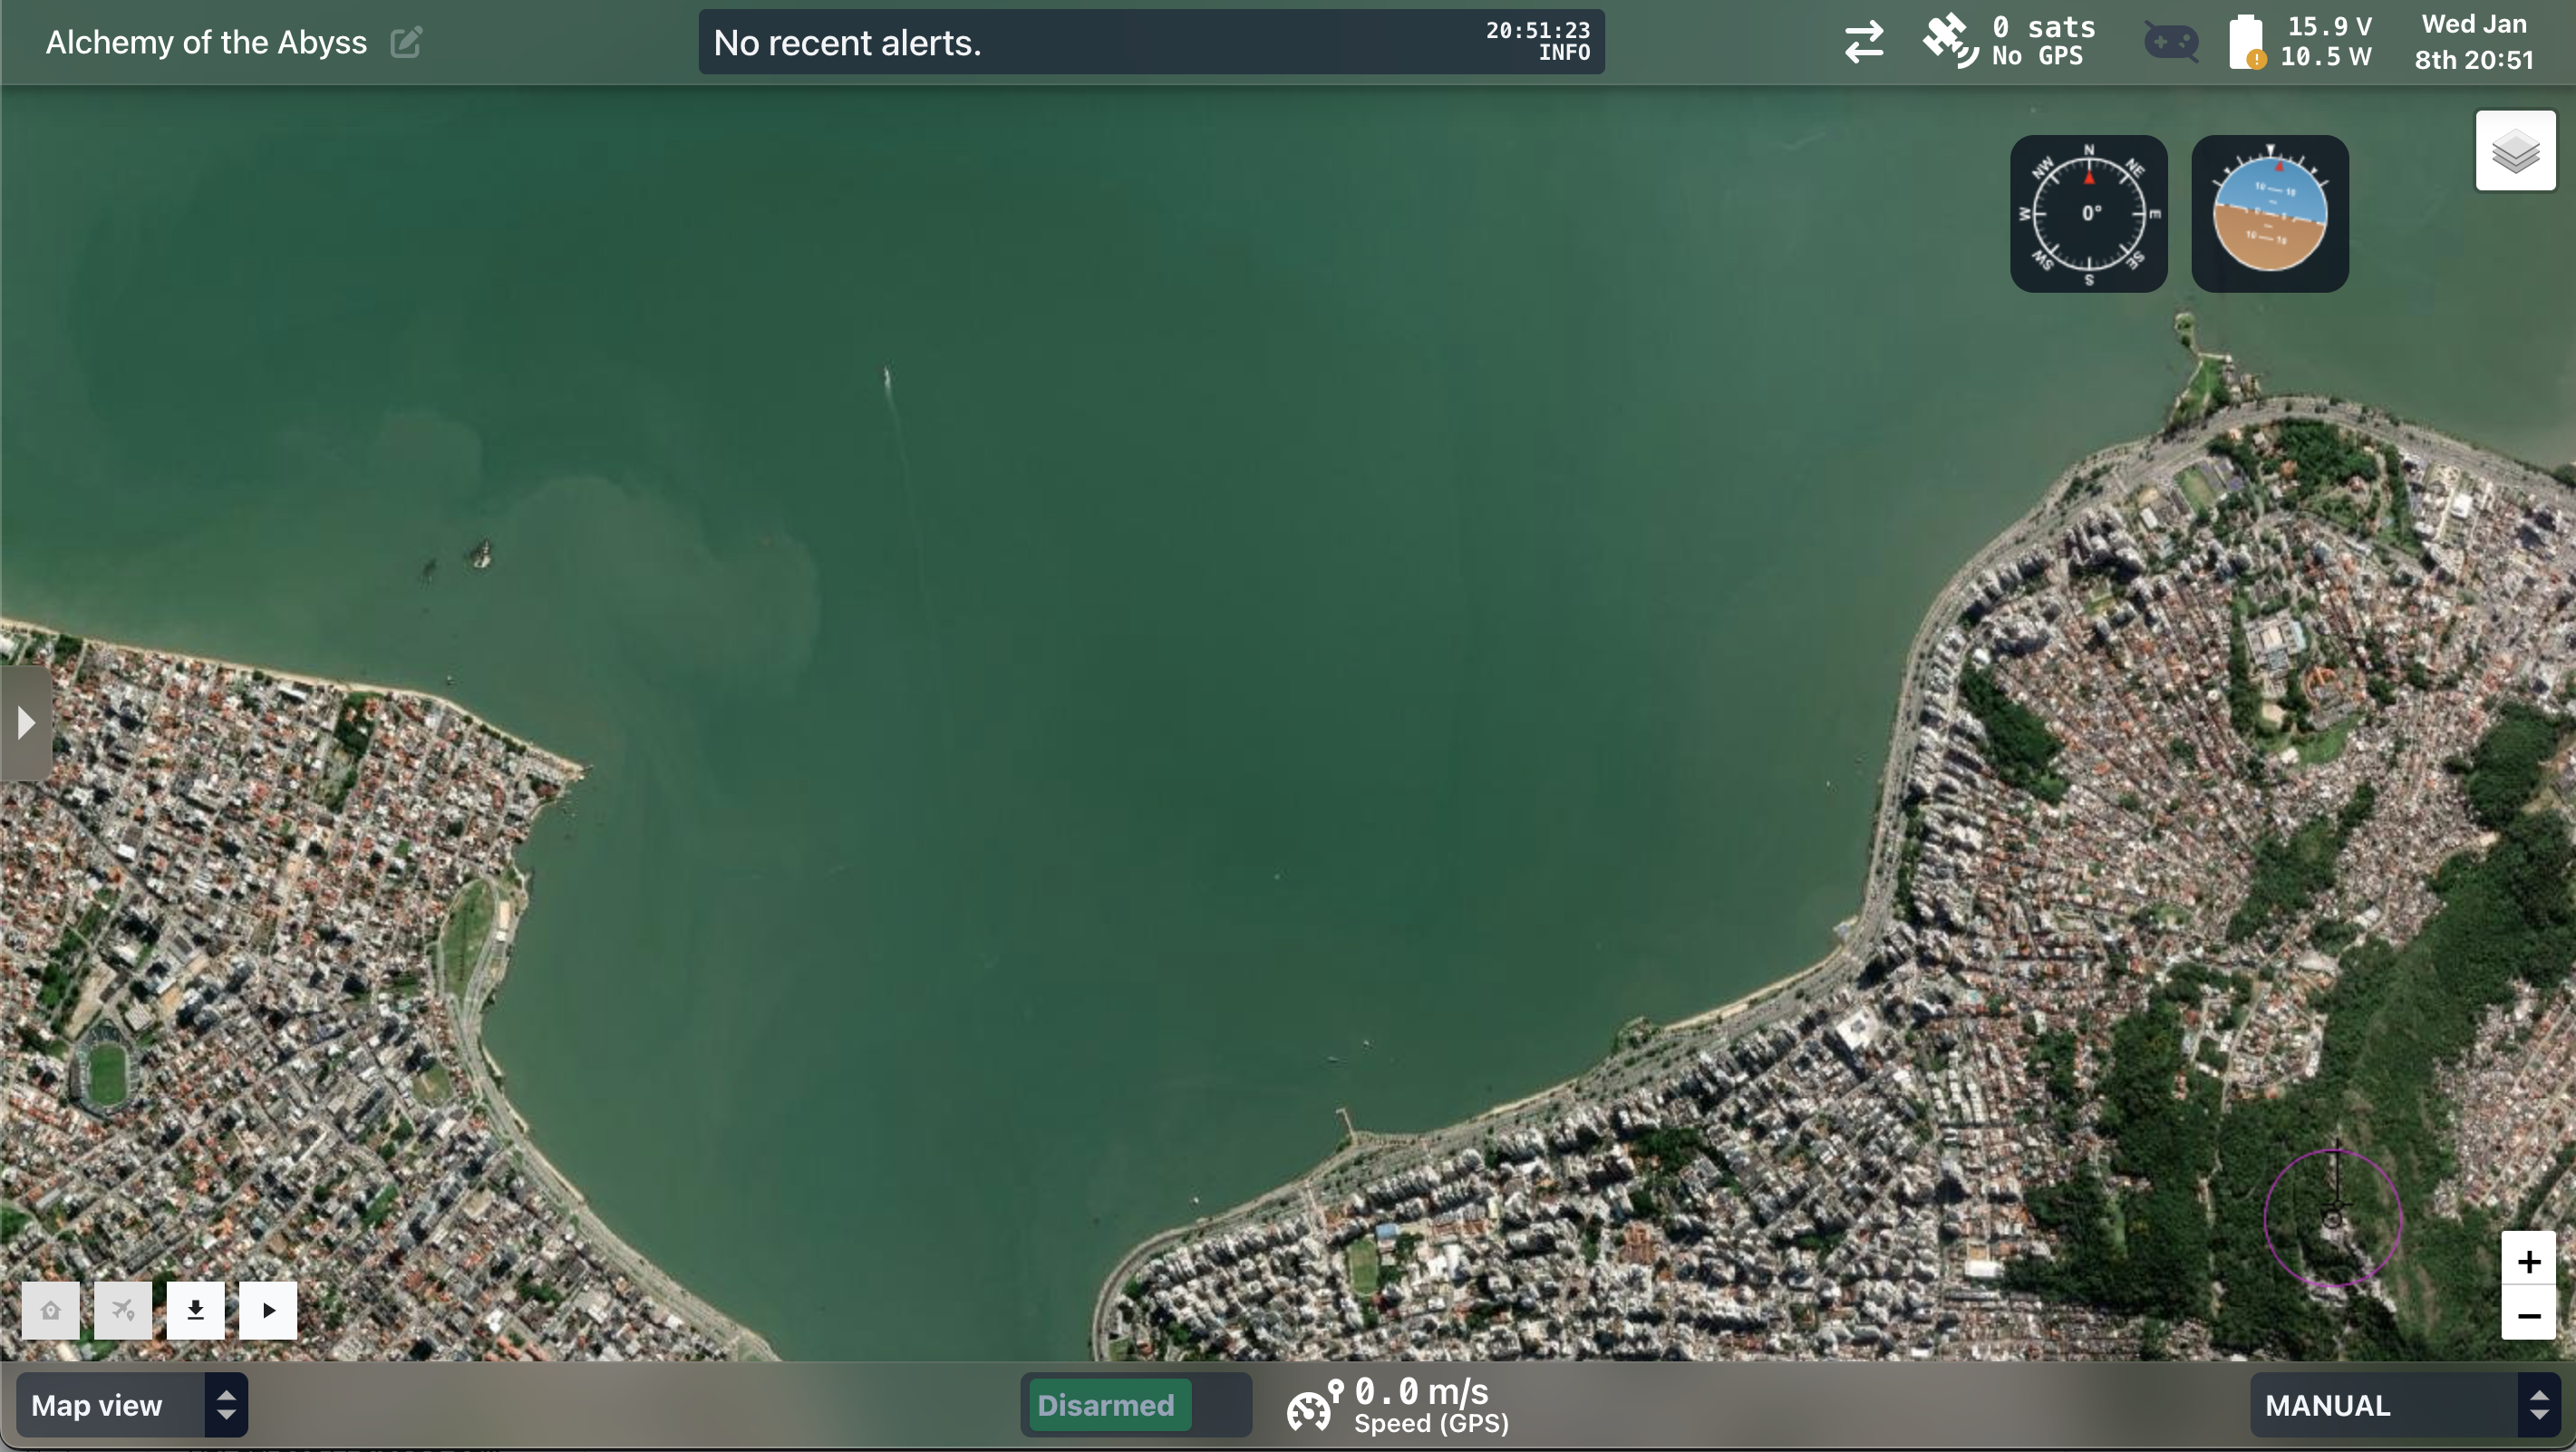
\includegraphics[width=\linewidth, height=2.35cm, keepaspectratio]{boat-map-view.png}\\
        \vspace{0.15em}
        \succw{Vue Cartographique ASV (BlueBoat)}\\
        \tiny\textit{Suivi de mission, géoréférencement GNSS RTK et bathymétrie}
      \end{center}
      \vspace{-0.4em}
      \begin{block}{Navigation \& Relevé Surfacique}
        \scriptsize
        \begin{itemize}
          \item \textbf{Fond de carte satellite} : centrage automatique sur la trace GPS haute précision du navire.
          \item \textbf{Planification autonome} : tracé de transects réguliers pour fauchée acoustique ou profils CTD.
          \item \textbf{Surveillance distante} : vitesse sol, satellites GNSS, télémétrie sol WiFi ($>500\,\text{m}$).
        \end{itemize}
      \end{block}
    \end{column}
  \end{columns}
\end{frame}
\begin{frame}{3.5 L'Intégration ROS / ROS 2 pour les Data Scientists}
  \begin{center}
    \begin{tikzpicture}[scale=0.85, auto, node distance=1.2cm, >=Latex]
      \node[draw=OceanMedium, fill=OceanMedium!15, rounded corners, rectangle, minimum width=2.6cm, align=center] (ardusub) {
        \textbf{ArduSub / Rover}\\
        \footnotesize MAVLink Stream
      };
      \node[draw=OceanDeep, fill=OceanDeep!20, rounded corners, rectangle, minimum width=2.8cm, align=center, right=1.2cm of ardusub] (mavros) {
        \textbf{Pont ROS 2}\\
        \footnotesize \code{mavros} ou micro-ROS
      };
      \node[draw=OceanGreen, fill=OceanGreen!15, rounded corners, rectangle, minimum width=3.4cm, align=center, right=1.2cm of mavros] (rostopics) {
        \textbf{Topics ROS 2}\\
        \footnotesize \code{/mavros/imu/data}\\
        \footnotesize \code{/mavros/local\_position}\\
        \footnotesize \code{/sensor/ocean\_ctd}
      };
      \node[draw=OceanCyan, fill=OceanCyan!20, line width=1.2pt, rounded corners, rectangle, minimum width=3.4cm, align=center, below=0.8cm of rostopics] (rosbag) {
        \textbf{Enregistrement ROSBAG2}\\
        \footnotesize Fichiers \textbf{.mcap} complets\\
        \footnotesize Horodatage nanoseconde
      };

      \draw[->, thick, OceanDeep] (ardusub) -- (mavros);
      \draw[->, thick, OceanDeep] (mavros) -- (rostopics);
      \draw[->, line width=1.5pt, OceanCyan] (rostopics) -- (rosbag);
    \end{tikzpicture}
  \end{center}

  \begin{block}{Pourquoi ROS 2 est l'outil ultime pour le traitement de données ?}
    \begin{itemize}
      \item \textbf{Synchronisation de messages (\code{message\_filters})} : fusionne automatiquement la navigation (DVL/IMU) et les mesures scientifiques au même instant $t$.
      \item \textbf{Gestion des repères spatiaux (\code{tf2})} : gère le bras de levier (*lever arm*) entre le centre de gravité, le DVL, la caméra et le capteur CTD.
    \end{itemize}
  \end{block}
\end{frame}

\begin{frame}{3.5b Logs Telemetry Dataflash (.bin), Rejeu \& UAV Log Viewer}
  \begin{columns}[T]
    \begin{column}{0.48\textwidth}
      \begin{block}{\tech{Les Logs Bruts Autopilote (.bin)}}
        \scriptsize
        \begin{itemize}
          \item ArduSub enregistre en continu des fichiers de télémétrie binaire Dataflash \code{.bin} directement sur la carte SD ou la mémoire Flash du calculateur (RPi/Navigator/Pixhawk).
          \item Contiennent \textbf{toutes les données internes à 50 Hz--400 Hz} : attitudes IMU, consignes moteurs PWM, profondeurs Bar30, états des fail-safes et pings DVL.
          \item Indispensables pour l'expertise post-incident et la reconstruction exacte de la plongée.
        \end{itemize}
      \end{block}

      \begin{block}{\succw{Rejeu \& Traitement Hors-Ligne}}
        \scriptsize
        \begin{itemize}
          \item \textbf{Rejeu MAVLink (QGC)} : rejouer la mission entière seconde par seconde comme en direct sur le terrain.
          \item \textbf{Pipeline Python (\code{pymavlink})} : export direct vers \code{pandas} / CSV pour traitement scientifique.
        \end{itemize}
      \end{block}
    \end{column}

    \begin{column}{0.48\textwidth}
      \begin{center}
        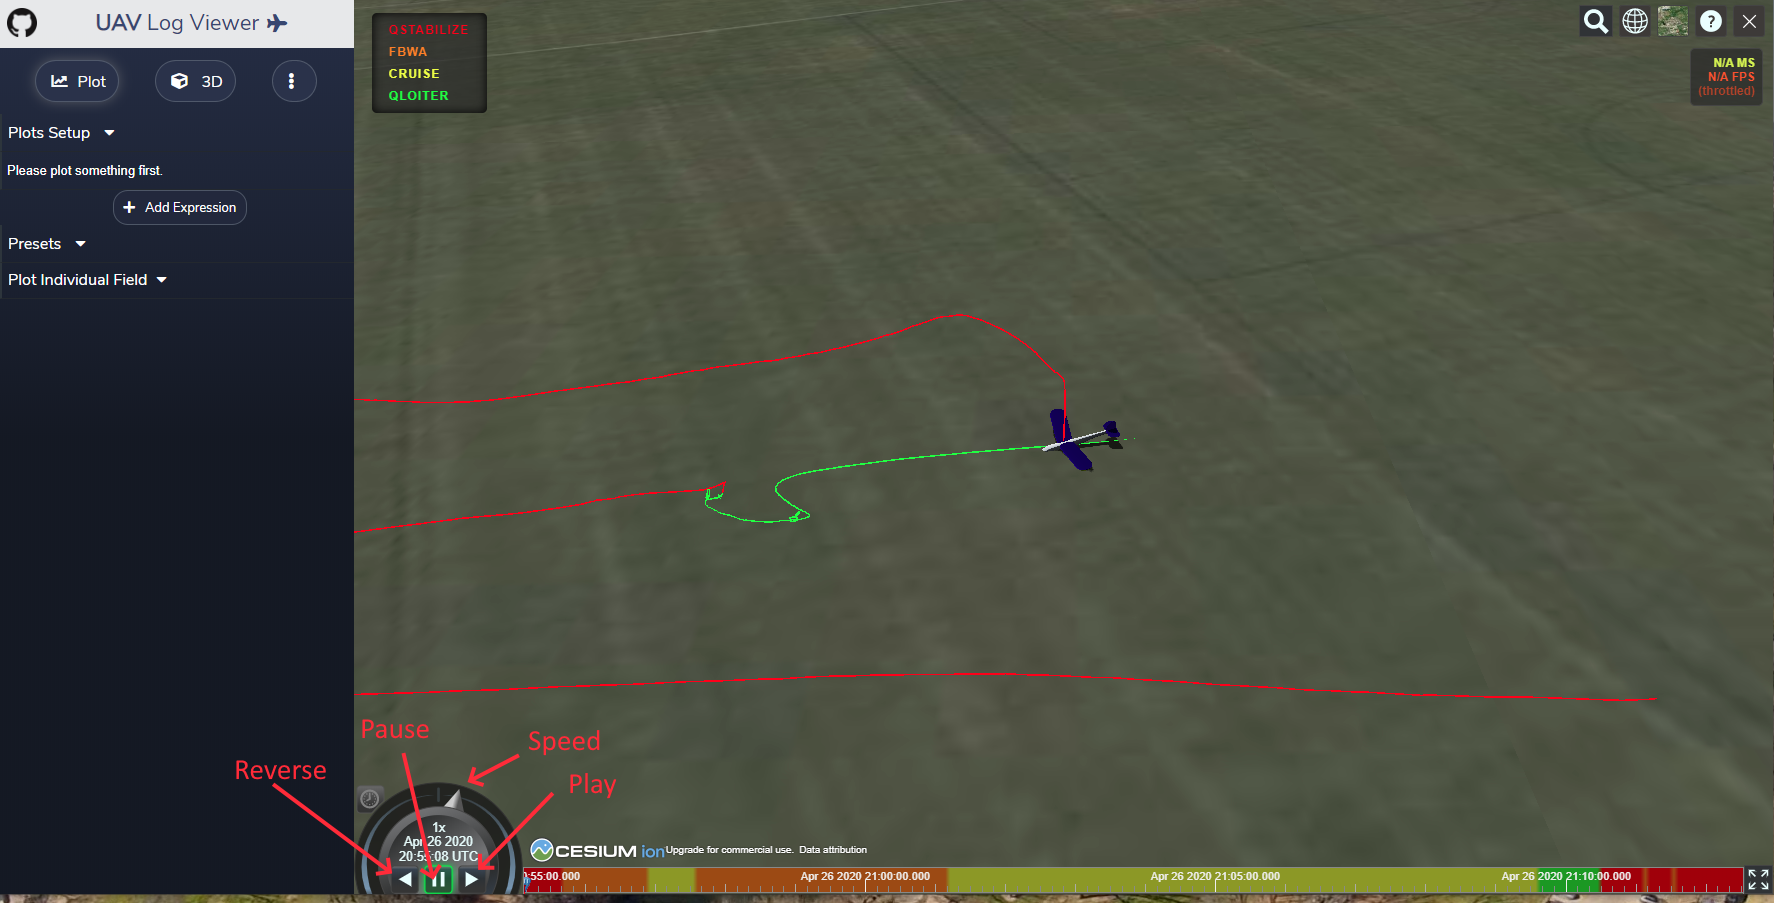
\includegraphics[width=\linewidth, height=2.6cm, keepaspectratio]{uav_logviewer.png}\\
        \vspace{0.15em}
        \succw{UAV Log Viewer (\href{https://plot.ardupilot.org}{\code{plot.ardupilot.org}})}\\
        \tiny\textit{Visualisation 3D, spectres de vibrations IMU \& analyse temporelle}
      \end{center}
      \vspace{-0.4em}
      \begin{block}{Diagnostic Visuel \& Rejeu en Ligne}
        \scriptsize
        \begin{itemize}
          \item \textbf{Zéro installation} : glisser-déposer direct du fichier \code{.bin} dans le navigateur web.
          \item \textbf{Trajectoire 3D dynamique} : suivi spatial synchronisé avec les graphes de capteurs (batterie, cap, profondeur).
          \item \textbf{Analyse fréquentielle (FFT)} : détection des résonances mécaniques et vibrations propulseurs.
        \end{itemize}
      \end{block}
    \end{column}
  \end{columns}
\end{frame}

\begin{frame}{3.6 Capteurs de Sûreté Véhicule \& Fail-Safes Réels}
  \begin{table}[h]
    \centering
    \scriptsize
    \begin{tabularx}{\textwidth}{l p{4.2cm} X}
      \toprule
      \textbf{Capteur de Sûreté} & \textbf{Principe \& Implantation} & \textbf{Réaction Automatique (Fail-Safe)} \\
      \midrule
      \alertw{SOS Leak Sensor} & Bandes conductimétriques au point le plus bas des caissons (électronique \& batterie) & Alerte sonore QGC/Cockpit, clignotement des feux Lumen, désarmement propulsion, remontée passive \\
      \alertw{Pression interne} & Surveillance de la dépression post-test de vide ($<-0.4\,\text{bar}$) & Détection d'infiltration d'air/eau \succw{avant tout contact liquide avec l'électronique} \\
      \alertw{Sonde Power Sense} & Mesure courant crête ($<60\,\text{A}$) et tension cellule Li-ion ($>3.3\,\text{V}$) & Alerte tension basse, coupure préventive des charges utiles secondaires \\
      \alertw{Heartbeat MAVLink} & Perte de communication ombilical ou WiFi ($>5\,\text{s}$) & Mode \textbf{Disarm} automatique, coupure moteurs et retour de surface par flottabilité positive \\
      \bottomrule
    \end{tabularx}
  \end{table}

  \begin{block}{\tech{Philosophie des Fail-Safes Réseau \& Matériels}}
    \scriptsize
    Chaque capteur de sûreté est relié à une boucle d'asservissement matérielle ou logicielle sous ArduSub/BlueOS. En cas de défaillance critique, le robot privilégie toujours sa \succw{remontée passive en surface} et la préservation de ses données embarquées.
  \end{block}
\end{frame}

\begin{frame}{3.6b Focus Matériel : Le SOS Leak Sensor}
  \begin{columns}[c]
    \begin{column}{0.40\textwidth}
      \begin{center}
        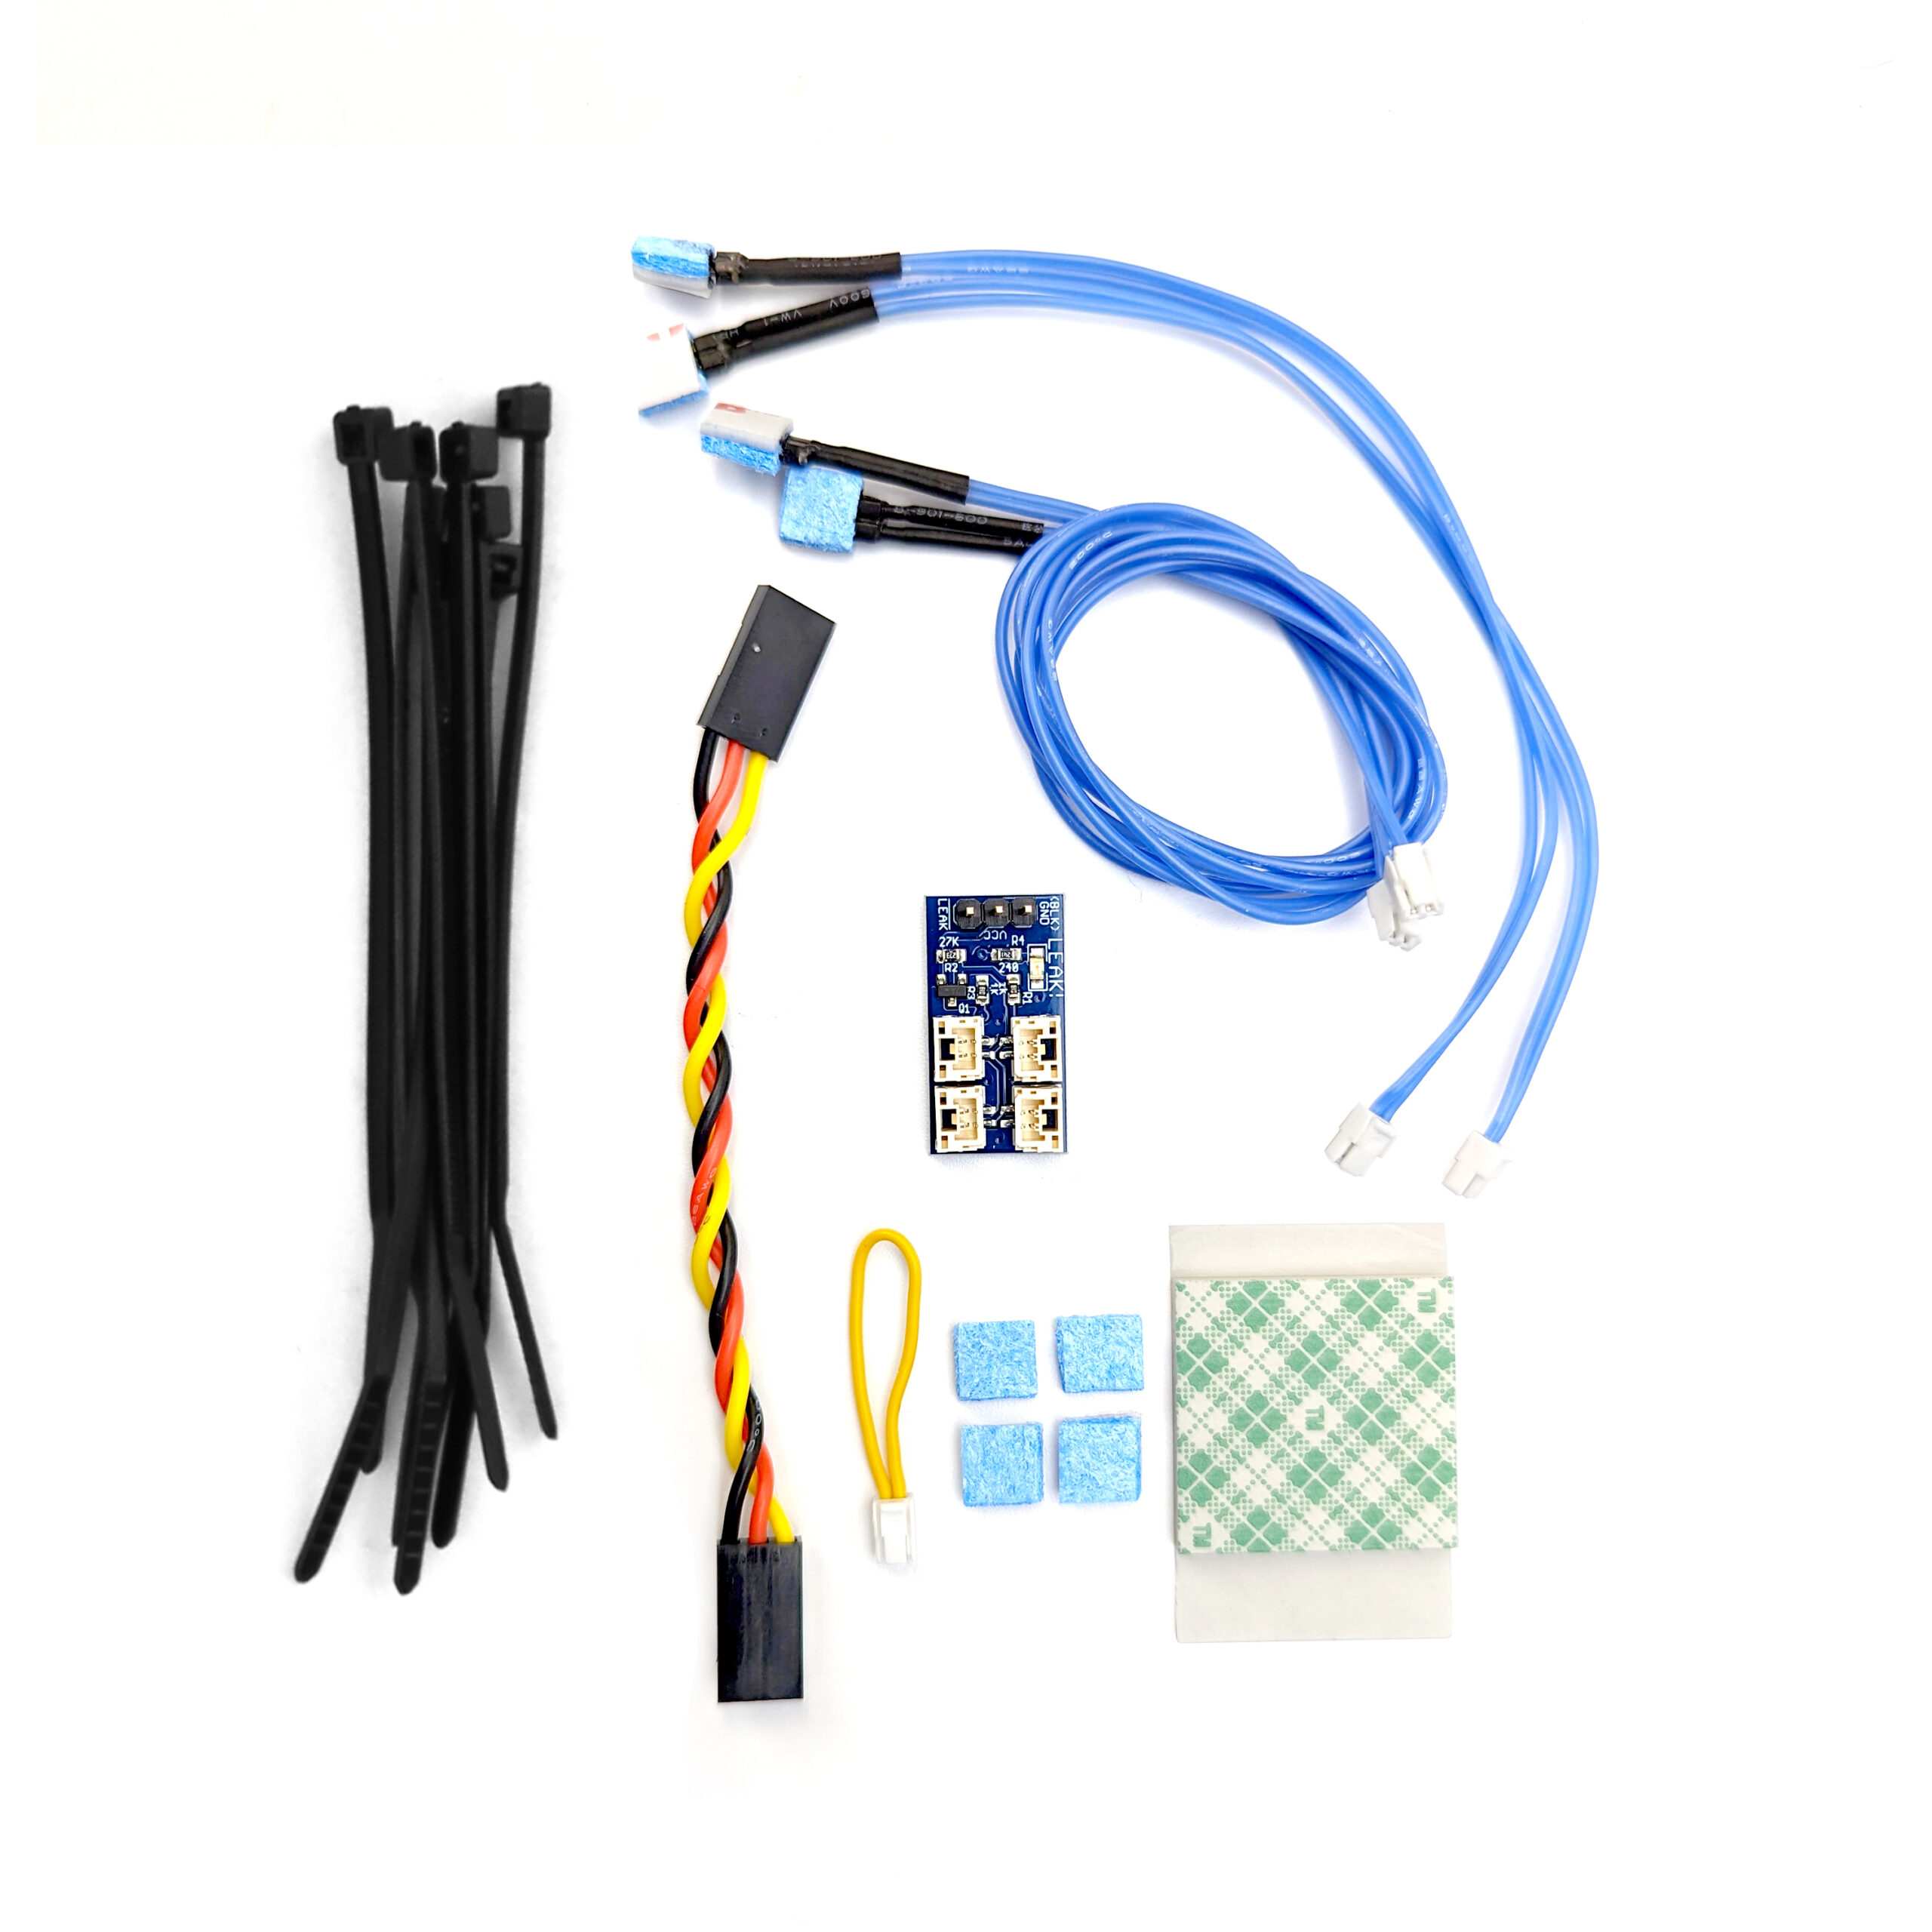
\includegraphics[height=3.4cm, keepaspectratio]{sos_leak_sensor.jpg}\\
        \vspace{0.2em}
        \footnotesize\textbf{BlueRobotics SOS Leak Sensor}\\
        \scriptsize\textit{Circuit comparateur \& sondes conductives}
      \end{center}
    \end{column}

    \begin{column}{0.58\textwidth}
      \begin{block}{\tech{Fonctionnement du SOS Leak Sensor}}
        \scriptsize
        \begin{itemize}
          \item Circuit comparateur connecté directement sur une entrée GPIO de l'autopilote (carte Navigator / Pixhawk).
          \item Rubans adhésifs à pistes interdigitées tapissant le fond du tube : la moindre goutte salée ou douce ferme le circuit par conduction.
          \item Déclenche l'alerte sonore Cockpit/QGC et le clignotement d'urgence des feux Lumen.
        \end{itemize}
      \end{block}
    \end{column}
  \end{columns}
\end{frame}
